% Soubory musí být v kódování, které je nastaveno v příkazu \usepackage[...]{inputenc}

\documentclass[%        Základní nastavení
%  draft,    				  % Testovací překlad
  12pt,       				% Velikost základního písma je 12 bodů
  a4paper,    				% Formát papíru je A4
  %oneside,      			% Jednostranný tisk
	twoside,      			% Dvoustranný tisk (kapitoly a další důležité části tedy začínají na lichých stranách)
	unicode,						% Záložky a metainformace ve výsledném  PDF budou v kódování unicode
]{report}				    	% Dokument třídy 'zpráva', vhodná pro sazbu závěrečných prací s kapitolami

\usepackage[utf8]		  %	Kódování zdrojových souborů je UTF-8
	{inputenc}					% Balíček pro nastavení kódování zdrojových souborů

\usepackage[				% Nastavení geometrie stránky
	bindingoffset=10mm,		% Hřbet pro vazbu
	hmargin={25mm,25mm},	% Vnitřní a vnější okraj
	vmargin={25mm,34mm},	% Horní a dolní okraj
	footskip=17mm,			  % Velikost zápatí
	nohead,					      % Bez záhlaví
	marginparsep=2mm,		  % Vzdálenost marginálií
	marginparwidth=18mm,	% Šířka marginálií
]{geometry}

\usepackage{sectsty}
	%přetypuje nadpisy všech úrovní na bezpatkové, kromě \chapter, která je přenastavena zvlášť v thesis.sty
	\allsectionsfont{\sffamily}

\usepackage{graphicx} % Balíček 'graphicx' pro vkládání obrázků
											% Nutné pro vložení logotypů školy a fakulty

\usepackage[          % Balíček 'acronym' pro sazby zkratek a symbolů
	nohyperlinks				% Nebudou tvořeny hypertextové odkazy do seznamu zkratek
]{acronym}						
											% Nutné pro použití prostředí 'acronym' balíčku 'thesis'

\usepackage[
	breaklinks=true,		% Hypertextové odkazy mohou obsahovat zalomení řádku
	hypertexnames=false % Názvy hypertext. odkazů budou tvořeny nezávisle na názvech TeXu
]{hyperref}						% Balíček 'hyperref' pro sazbu hypertextových odkazů
											% Nutné pro použití příkazu 'pdfsettings' balíčku 'thesis'

\usepackage{pdfpages} % Balíček umožňující vkládat stránky z PDF souborů
                      % Nutné při vkládání titulních listů a zadání přímo
                      % ve formátu PDF z informačního systému

\usepackage{enumitem} % Balíček pro nastavení mezerování v odrážkách
  \setlist{topsep=0pt,partopsep=0pt,noitemsep} % konkrétní nastavení

\usepackage{cmap} 		% Balíček cmap zajišťuje, že PDF vytvořené `pdflatexem' je
											% plně "prohledávatelné" a "kopírovatelné"

%\usepackage{upgreek}	% Balíček pro sazbu stojatých řeckých písmem
											%% např. stojaté pí: \uppi
											%% např. stojaté mí: \upmu (použitelné třeba v mikrometrech)
											%% pozor, grafická nekompatibilita s fonty typu Computer Modern!
                      
%\usepackage{amsmath} %balíček pro sabu náročnější matematiky                 

\usepackage{dirtree}	% sazba adresářové struktury
                      % vhodné pro prezentaci obsahu elektronické přílohy (např. CD)

\usepackage[formats]{listings}	% Balíček pro sazbu zdrojových textů
\lstset{              % nastavení
%	Definice jazyka použitého ve výpisech
%    language=[LaTeX]{TeX},	% LaTeX
%	language={Matlab},		% Matlab
	language={C},           % jazyk C
    basicstyle=\ttfamily,	% definice základního stylu písma
    tabsize=2,			% definice velikosti tabulátoru
    inputencoding=utf8,         % pro soubory uložené v kódování UTF-8
		columns=fixed,  %fixed nebo flexible,
		fontadjust=true %licovani sloupcu
    extendedchars=true,
    literate=%  definice symbolů s diakritikou
    {á}{{\'a}}1
    {č}{{\v{c}}}1
    {ď}{{\v{d}}}1
    {é}{{\'e}}1
    {ě}{{\v{e}}}1
    {í}{{\'i}}1
    {ň}{{\v{n}}}1
    {ó}{{\'o}}1
    {ř}{{\v{r}}}1
    {š}{{\v{s}}}1
    {ť}{{\v{t}}}1
    {ú}{{\'u}}1
    {ů}{{\r{u}}}1
    {ý}{{\'y}}1
    {ž}{{\v{z}}}1
    {Á}{{\'A}}1
    {Č}{{\v{C}}}1
    {Ď}{{\v{D}}}1
    {É}{{\'E}}1
    {Ě}{{\v{E}}}1
    {Í}{{\'I}}1
    {Ň}{{\v{N}}}1
    {Ó}{{\'O}}1
    {Ř}{{\v{R}}}1
    {Š}{{\v{S}}}1
    {Ť}{{\v{T}}}1
    {Ú}{{\'U}}1
    {Ů}{{\r{U}}}1
    {Ý}{{\'Y}}1
    {Ž}{{\v{Z}}}1
}

%%%%%%%%%%%%%%%%%%%%%%%%%%%%%%%%%%%%%%%%%%%%%%%%%%%%%%%%%%%%%%%%%
%%%%%%      Definice informací o dokumentu             %%%%%%%%%%
%%%%%%%%%%%%%%%%%%%%%%%%%%%%%%%%%%%%%%%%%%%%%%%%%%%%%%%%%%%%%%%%%

% V tomto souboru se nastavují téměř veškeré informace, proměnné mezi studenty:
% jméno, název práce, pohlaví atd.
% Tento soubor je SDÍLENÝ mezi textem práce a prezentací k obhajobě -- netřeba něco nastavovat na dvou místech.

\usepackage[
%%% Z následujících voleb jazyka lze použít pouze jednu
  czech-english,		% originální jazyk je čeština, překlad je anglicky (výchozí)
  %english-czech,	% originální jazyk je angličtina, překlad je česky
  %slovak-english,	% originální jazyk je slovenština, překlad je anglicky
  %english-slovak,	% originální jazyk je angličtina, překlad je slovensky
%
%%% Z následujících voleb typu práce lze použít pouze jednu
  semestral,		  % semestrální práce (nesází se abstrakty, prohlášení, poděkování) (výchozí)
  %bachelor,			%	bakalářská práce
  %master,			  % diplomová práce
  %treatise,			% pojednání o disertační práci
  %doctoral,			% disertační práce
%
%%% Z následujících voleb zarovnání objektů lze použít pouze jednu
%  left,				  % rovnice a popisky plovoucích objektů budou zarovnány vlevo
	center,			    % rovnice a popisky plovoucích objektů budou zarovnány na střed (vychozi)
%
]{thesis}   % Balíček pro sazbu studentských prací

\usepackage{microtype}

%%% Jméno a příjmení autora ve tvaru
%  [tituly před jménem]{Křestní}{Příjmení}[tituly za jménem]
% Pokud osoba nemá titul před/za jménem, smažte celý řetězec '[...]'
\author[Bc.]{Renata}{Zemanová}

%%% Identifikační číslo autora (VUT ID)
\butid{211251}

%%% Pohlaví autora/autorky
% (nepoužije se ve variantě english-czech ani english-slovak)
% Číselná hodnota: 1...žena, 0...muž
\gender{1}

%%% Jméno a příjmení vedoucího/školitele včetně titulů
%  [tituly před jménem]{Křestní}{Příjmení}[tituly za jménem]
% Pokud osoba nemá titul před/za jménem, smažte celý řetězec '[...]'
\advisor[doc.\ Ing.]{Pavel}{Šteffan}[Ph.D.]

%%% Jméno a příjmení oponenta včetně titulů
%  [tituly před jménem]{Křestní}{Příjmení}[tituly za jménem]
% Pokud osoba nemá titul před/za jménem, smažte celý řetězec '[...]'
% Nastavení oponenta se uplatní pouze v prezentaci k obhajobě;
% v případě, že nechcete, aby se na titulním snímku prezentace zobrazoval oponent, pouze příkaz zakomentujte;
% u obhajoby semestrální práce se oponent nezobrazuje (jelikož neexistuje)
% U dizertační práce jsou typicky dva až tři oponenti. Pokud je chcete mít na titulním slajdu, prosím ručně odkomentujte a upravte jejich jména v definici "VUT title page" v souboru thesis.sty.
\opponent[doc.\ Mgr.]{Křestní}{Příjmení}[Ph.D.]

%%% Název práce
%  Parametr ve složených závorkách {} je název v originálním jazyce,
%  parametr v hranatých závorkách [] je překlad (podle toho jaký je originální jazyk).
%  V případě, že název Vaší práce je dlouhý a nevleze se celý do zápatí prezentace, použijte příkaz
%  \def\insertshorttitle{Zkác.\ náz.\ práce}
%  kde jako parametr vyplníte zkrácený název. Pokud nechcete zkracovat název, budete muset předefinovat,
%  jak se vytváří patička slidu. Viz odkaz: https://bit.ly/3EJTp5A
\title[Traffic light - technological equivalent of a streamer]{Semafor - technologický ekvivalent fáborku}

%%% Označení oboru studia
%  Parametr ve složených závorkách {} je název oboru v originálním jazyce,
%  parametr v hranatých závorkách [] je překlad
\specialization[Microelectronics]{Mikroelektronika}

%%% Označení ústavu
%  Parametr ve složených závorkách {} je název ústavu v originálním jazyce,
%  parametr v hranatých závorkách [] je překlad
%\department[Department of Control and Instrumentation]{Ústav automatizace a měřicí techniky}
%\department[Department of Biomedical Engineering]{Ústav biomedicínského inženýrství}
%\department[Department of Electrical Power Engineering]{Ústav elektroenergetiky}
%\department[Department of Electrical and Electronic Technology]{Ústav elektrotechnologie}
%\department[Department of Physics]{Ústav fyziky}
%\department[Department of Foreign Languages]{Ústav jazyků}
%\department[Department of Mathematics]{Ústav matematiky}
\department[Department of Microelectronics]{Ústav mikroelektroniky}
%\department[Department of Radio Electronics]{Ústav radioelektroniky}
%\department[Department of Theoretical and Experimental Electrical Engineering]{Ústav teoretické a experimentální elektrotechniky}
%\department[Department of Telecommunications]{Ústav telekomunikací}
%\department[Department of Power Electrical and Electronic Engineering]{Ústav výkonové elektrotechniky a elektroniky}

%%% Označení fakulty
%  Parametr ve složených závorkách {} je název fakulty v originálním jazyce,
%  parametr v hranatých závorkách [] je překlad
%\faculty[Faculty of Architecture]{Fakulta architektury}
\faculty[Faculty of Electrical Engineering and~Communication]{Fakulta elektrotechniky a~komunikačních technologií}
%\faculty[Faculty of Chemistry]{Fakulta chemická}
%\faculty[Faculty of Information Technology]{Fakulta informačních technologií}
%\faculty[Faculty of Business and Management]{Fakulta podnikatelská}
%\faculty[Faculty of Civil Engineering]{Fakulta stavební}
%\faculty[Faculty of Mechanical Engineering]{Fakulta strojního inženýrství}
%\faculty[Faculty of Fine Arts]{Fakulta výtvarných umění}
%
%Nastavení logotypu (v hranatych zavorkach zkracene logo, ve slozenych plne):
\facultylogo[logo/FEKT_zkratka_barevne_PANTONE_CZ]{logo/UTKO_color_PANTONE_CZ}

%%% Rok odevzdání práce
\graduateyear{2023}
%%% Akademický rok odevzdání práce
\academicyear{2022/23}

%%% Datum obhajoby (uplatní se pouze v prezentaci k obhajobě)
\date{11.\,01.\,2023} 

%%% Místo obhajoby
% Na titulních stránkách bude automaticky vysázeno VELKÝMI písmeny (pokud tyto stránky sází šablona)
\city{Brno}

%%% Abstrakt
\abstract[%
The goal of this semestral thesis is to design device called Traffic light, which serves as an assistant in outdoor games and for education
purposes. The design focuses on safety, simplicity and low cost. 

This thesis deals with the selection and design of the overall electronics contained in the Traffic light. Emphasis is placed on the selection 
of the light signaling, wireless module and microcontroller.
]{%
Cílem práce je navrhnout elektronické zařízení Semafor, který slouží jako pomocník při outdoorových hrách a pro edukační účely. 
Při návrhu je kladen důraz na bezpečnost, jednoduchost a nízkou cenu. 

Tato práce se zabývá výběrem a návrhem celkové elektroniky, kterou Semafor obsahuje. Je kladen důraz na výběr světelné signalizace, 
bezdrátového modulu a mikrokontroléru. 
}

%%% Klíčová slova
\keywrds[%
Traffic light, microcontroller, programmable LED WS2812C, batteries LiFePO4, LoRa module, capacitive touch buttons
]{%
Semafor, mikrokontrolér, programovatelné LED WS2812C, baterie LiFePO4, LoRa modul, kapacitní dotyková tlačítka
}

%%% Poděkování
\acknowledgement{%
Ráda bych poděkovala vedoucímu diplomové práce panu doc. Ing.~Pavlovi Šteffanovi, Ph.D.\ za odborné vedení,
konzultace, podnětné návrhy k~práci a zapůjčení testovacího hardwaru. Dále také děkuji RNDr. Janovi Mrázkovi 
za podnětné rady při návrhu elektroniky. 
}%  % do tohoto souboru doplňte údaje o sobě, druhu práce, názvu...

%%%%%%%%%%%%%%%%%%%%%%%%%%%%%%%%%%%%%%%%%%%%%%%%%%%%%%%%%%%%%%%%%%%%%%%%

%%%%%%%%%%%%%%%%%%%%%%%%%%%%%%%%%%%%%%%%%%%%%%%%%%%%%%%%%%%%%%%%%%%%%%%%
%%%%%%     Nastavení polí ve Vlastnostech dokumentu PDF      %%%%%%%%%%%
%%%%%%%%%%%%%%%%%%%%%%%%%%%%%%%%%%%%%%%%%%%%%%%%%%%%%%%%%%%%%%%%%%%%%%%%
%% Při načteném balíčku 'hyperref' lze použít příkaz '\pdfsettings':
\pdfsettings
%  Nastavení polí je možné provést také ručně příkazem:
%\hypersetup{
%  pdftitle={Název studentské práce},    	% Pole 'Document Title'
%  pdfauthor={Autor studenstké práce},   	% Pole 'Author'
%  pdfsubject={Typ práce}, 						  	% Pole 'Subject'
%  pdfkeywords={Klíčová slova}           	% Pole 'Keywords'
%}
%%%%%%%%%%%%%%%%%%%%%%%%%%%%%%%%%%%%%%%%%%%%%%%%%%%%%%%%%%%%%%%%%%%%%%%

\pdfmapfile{=vafle.map}

%%%%%%%%%%%%%%%%%%%%%%%%%%%%%%%%%%%%%%%%%%%%%%%%%%%%%%%%%%%%%%%%%%%%%%%
%%%%%%%%%%%       Začátek dokumentu               %%%%%%%%%%%%%%%%%%%%%
%%%%%%%%%%%%%%%%%%%%%%%%%%%%%%%%%%%%%%%%%%%%%%%%%%%%%%%%%%%%%%%%%%%%%%%
\begin{document}
\pagestyle{empty} %vypnutí číslování stránek

%%% Vložení desek -- od září 2021 na žádost fakulty nepoužíváno
%\includepdf[pages=1]%  buďto generovaných informačním systémem
  %{pdf/student-desky}% název souboru nesmí obsahovat mezery!
%%% NEBO vytvoření desek z balíčku
%%\makecover
%%%
%\oddpage % při dvojstranném tisku přidá prázdnou stránku
%% kazdopádně ale:
%\setcounter{page}{1} %resetovaní čítače stránek -- desky do číslování nezahrnujeme

\includepdf[pages=1]%    buďto generovaného informačním systémem
  {pdf/Desky}

%% Vložení titulního listu
\includepdf[pages=1]%    buďto generovaného informačním systémem
  {pdf/Titulni_strana_barevne}% název souboru nesmí obsahovat mezery!
%% NEBO vytvoření titulní stránky z balíčku
%\maketitle
%%
%\oddpage  % při dvojstranném tisku se přidá prázdná stránka
   
%% Vložení zadání
\includepdf[pages=1]%   buďto generovaného informačním systémem
  {pdf/Zadani_CZ_barevne}% název souboru nesmí obsahovat mezery!
%% NEBO lze vytvořit prázdný list příkazem ze šablony
%\patternpage{}%
%	{\sffamily\Huge\centering ZDE VLOŽIT LIST ZADÁNÍ}%
%	{\sffamily\centering Z~důvodu správného číslování stránek}
%%
%\oddpage% při dvojstranném tisku se přidá prázdná stránka

%% Vysázení stránky s abstraktem
\makeabstract

% Vysázení stránky s rozšířeným abstraktem
% (pokud píšete práci v češtině či slovenštině, vložení rozšířeného abstraktu zrušte;
%  pro semestrální projekt také není potřeba rozšířený abstrakt uvádět)
%% Vysázení stránky s rozšířeným abstraktem
% (týká se pouze bc. a dp. prací psaných v angličtině, viz Směrnice rektora 72/2017)
\cleardoublepage
\noindent
{\large\sffamily\bfseries\MakeUppercase{Rozšířený abstrakt}}
\\
Výtah ze směrnice rektora 72/2017:\\
\emph{Bakalářská a diplomová práce předložená v angličtině musí obsahovat rozšířený abstrakt v češtině
nebo slovenštině (čl. 15). To se netýká studentů, kteří studují studijní program akreditovaný v
angličtině.}
(čl. 3, par. 7)\\
\emph{Nebude-li vnitřní normou stanoveno jinak, doporučuje se rozšířený abstrakt o rozsahu přibližně 3
normostrany, který bude obsahovat úvod, popis řešení a shrnutí a zhodnocení výsledků.}
(čl. 15, par. 5)

%%% Vysázení citace práce
\makecitation

%%% Vysázení prohlášení o samostatnosti
\makedeclaration

%%% Vysázení poděkování
\makeacknowledgement

%%% Vysázení obsahu
\tableofcontents

\cleardoublepage\pagestyle{plain}   % zapnutí číslování stránek

%Pro vkládání kapitol i příloh používejte raději \include než \input
%%% Vložení souboru 'text/uvod.tex' s úvodem
\chapter*{Úvod}
\phantomsection
\addcontentsline{toc}{chapter}{Úvod}

Tato práce se zabývá návrhem zařízení Semafor. Semafor slouží jako pomocník pro táborové hry nebo pro edukační účely. Je kladen důraz na co 
nejširší možnosti využití. Může plnit funkci například zástupu organizátora na stanovišti nebo fáborku pro určení směru, kam jít, a mnoho 
dalších. Pomocí dotykových senzorů lze zadávat kódy a na základě správného zadání lze získávat potřebné informace pro dokončení úkolu. Dotykové
senzory také slouží pro konfiguraci a nastavení funkce samotného semaforu. Informace o~stavu Semaforu, o~průběhu hry, o~správnosti kódu a podobně
jsou předávány pomocí světelných, zvukových a vibračních signalizací. 

Semafor je tedy navrhován pro outdoorové aplikace. Proto je kladen důraz na kompaktnost, bezpečnost, nízkou cenu, nízkou spotřebu a jednoduchost, 
aby s~ním mohl manipulovat pouhý laik, který má k~tomuto zařízení návod. Celý návrh je také koncipován tak, aby bylo možné zaručit voděodolnost 
výsledného zařízení. 

Základními požadavky na funkci Semaforu je, aby mohl svítit různými barvami, proto je část práce věnována právě výběru součástek pro světelnou 
signalizaci. Dotykové senzory jsou vybírány dle požadavku na spolehlivost, cenu a možnost voděodolnosti.

Dalším požadavkem pro rozšíření možností her je, aby Semafory mohly komunikovat mezi sebou. Mohou si tak předávat informace o~aktuální svítící 
barvě nebo stisknutém tlačítku. 

Semafor je řízen mikrokontrolérem, proto je část práce věnována jeho výběru. Nemalá část je také věnována výběru typu napájení Semaforu vzhledem 
k~použití na táborech a venkovních akcích.  

Semafory musí být také jednoduše konfigurovatelné, aby mohl běžný laik nastavit konkrétní hru, její parametry a vše bez problémů spustit. 





%%% Vložení souboru 'text/cile.tex' s úvodem
\chapter*{Cíle práce}
\phantomsection
\addcontentsline{toc}{chapter}{Cíle práce}

Konkrétní specifikace cílů, které má autor v~práci vyřešit.
Tato kapitola je \emph{volitelná} -- pokud váš studijní program nevyžaduje zvláštní kapitolu s cíli,
cíle specifikujte v~rámci Úvodu.

%%% Vložení souboru 'text/reseni' s popisem řešení práce
% (rozdělte na více souborů či kapitol, pokud je vhodné)
\chapter{Požadavky}
voděodolnost


\chapter{Základní návrh}
%tady musí být text
%bude tady také blokové schéma

\section{Mikrokontrolér}
Rozsah napájecího napětí je 3 až 3,6 V \cite{ESP_C3_dtsh}.

\section{LED}
Jendím z nejdůležitějších požadavků na Semafor je, aby mohl svítit. Čím více možností, jak svítit, tím bude využití 
při hrách a táborových programech větší. K tomu jsou použity LED. Obyčejné LED mají pouze jednu barvu, kterou 
mohou svítit. Existují také RBG LED, ale ty mají 4 vývody a každá LED tak zabírá 3 GPIO piny mikrokontroléru - jeden pin
pro jednu barvu. K tomu by byl zapotřebí mikrokonrolér s velkým množství GPIO pinů a jeho programování by se tím značně 
komplikovalo. Ani to není žádoucí, a proto byly použity programovatelné LED typu WS2812C. %citace

%způsob programování (jak funguje použitá knihovna?)

Tyto programovatelné LED WS2812C lze spojovat za sebe, takže datový výstup jedné LED je připojen k datovému vstupu další LED %citace
Takto lze spojit nekonečné množství těchto programovatelných LED. 

%obrázek spojení LED za sebe

%napsat o jejich spotřebě
%spočítat, jakou budou mít spotřebu celkem (všech 12) při bílé

%do sekce o DPS se zmínit o jejich umístění - kruh, hodiny, proto 12 ks. (lze také rozdělit na 3 segmenty)

\section{Tlačítka}
Tlačítka mohou být realizována dvěma základními způsoby, mohou být elektromechanická, nebo kapacitní dotyková. 

Dotyková plocha mechanického tlačítka je nevodivá, často plastová. 

Mechanické tlačítko typu NO: %upravit

Po zmáčknutí mechanického tlačítka jsou 2 kovové části tlačítka spojeny, tím dochází ke spojení elektrického obvodu 
a odpor smyčky je v ideálním případě nulový. Tlačítko je tedy sepnuto. Když je tlačítko rozpojeno, tak je 
elektrický obvod přerušen a odpor smyčky je v ideálním případě nekonečný.

Mechanické tlačítko typu NC: %upravit

U tlačítka NC je to přesně naopak. %upravit

%sem přidat fotku vnitřku mechanického tlačítka

Kapacitní tlačítka jsou tvořena měděnou vrstvou a nejsou nijak mechanicky namáhána. Tlačítko může být zmáčknuto i přes 
obal krabičky, a proto může být celé zařízení mechanicky odolné i voděodolné. 

Nevýhodou kapacitních tlačítek je, že nemají žádnou odezvu na dotyk. U mechanických tlačítek je odezvou samotný fyzický 
stisk tlačítka. U kapacitních tlačítek lze tento fakt vyřešit například rozsvícením LED nebo vibrační odezvou. Vibrační 
odezva může být realizována pomocí vibračního motoru. Některé MCU včetně vybraného mikrokontroléru ESP32-C3 nemají kapacitní
vstupy, to znamená, že tlačítko nelze připojit přímo k pinu MCU. Buď musí být vybrán mikrokonrolér, který kapacitní vstupy má,
nebo může být použit převodník, který má kapacitní vstupy a jeho výstupy poté mohou být připojeny k MCU. 

V návrhu Semaforu byla zvolena kapacitní dotyková tlačítka. Pro možnost použití uvnitř i venku jsou díky možnosti voděodolnosti 
vhodnějším řešením. Také označení tlačítka může být variabilní, protože může být na DPS v místě tlačítka vyznačeno barevně, nebo 
např. samolepkou. Odezva na dotyk se realizuje pomocí vibračního motoru. Ke čtení dotykových tlačítek je využit převodník. 
%realizace velikosti, proč centrální tlačítko větší

\subsection{Princip kapacitních dotykových tlačítek}
Základní princip je založen na měření změny kapacity. Měď, ze které je tlačítko vytvořeno má
nějakou vlastní kapacitu (kapacita samotné nosné desky) a po přiložení prstu je kapacita zvýšena o paralelně 
připojenou kapacitu přechodu tlačítka a prstu díky obsahu železa v krvi a vodivosti kůže \cite{PrincipKapTl}. 
Prst se tedy chová jako druhá uzemněná elektroda \cite{PrincipKapTl}. 

Kapacita snímače se tedy volí co nejmenší, aby přiložený prst vyvolal co nejvetší změnu kapacity. Ve snímači se vyskytuje
RC článek, kterého se mění doba nabíjení kondenzátoru a tím je možné detekovat stisk tlačítka \cite{PrincipKapTl}. 

\subsection{Návrh kapacitního dotykového tlačítka}
Tvar tlačítka nemá vliv na schopnost detekce dotyku \cite{PrincipKapTl}. Naopak velký vliv má plocha tlačítka, tloušťka
izolační vrstvy, a také vzdálenost jednotlivých tlačítek od sebe \cite{PrincipKapTl}. 

Čím větší je plocha tlačítka, tím je větší změna kapacity při dotyku a díky tomu je vytvořena lepší schopnost detekce 
dotyku \cite{PrincipKapTl}. S rostoucí tloušťkou izolační vrstvy se naopak schopnost detekce dotyku snižuje \cite{PrincipKapTl}.

Pokud jsou tlačítka příliš blízko u sebe, tak může docházet k jejich vzájemnému ovlivňování. Kvůli tomu pak může docházet k
detekci dotyku špatného tlačítka, nebo k falešné detekci dotyku. Z doporučení plyne, že pro dotyk prstu je vhodná velikost snímací 
plochu pro prst 13~$\times$~13 mm a jejich vzdálenost alespoň 5 mm od sebe \cite{PrincipKapTl}. Proti vzájemnému ovlivňování tlačítek
se používají uzemňovací meziplošky \cite{PrincipKapTl}. 

%sem dát obrázek, kde je ukázán návrh GND meziplošek

U kapacitních dotykových tlačítek je zapotřebí dbát na správné připojení k MCU. U vícevrstvých DPS nesmí pod tlačítky, ani pod přívody
k MCU, vést jiné dráhy, ani se zde nesmí vyskytovat jiné součástky \cite{PrincipKapTl}. Součástky nesmí být ani z vrchní, ani ze spodní 
strany DPS \cite{PrincipKapTl}. Přívody kapacitních tlačítek k MCU by měly být odstíněny pomocí GND signálu.

Voda a další nečistoty mění vlastní kapacitu tlačítka a může tak docházet k falešným stiskům tlačítka. Tento problém lze řešit softwarově. 
Lze využít faktu, že nečistoty působí dlouhodobě, ale stisk je krátkodobý \cite{PrincipKapTl}. Hodnotu vlastní kapacity tlačítka je tedy
možné softwarově upravovat v závislosti na aktuálních dlouhodobějších stavech a detekovat tak přesněji krátkodobý stisk tlačítka.

%dát do zkratek MCU, DPS, GPIO, LED, GND

\begin{figure}[!h]
    \begin{center}
      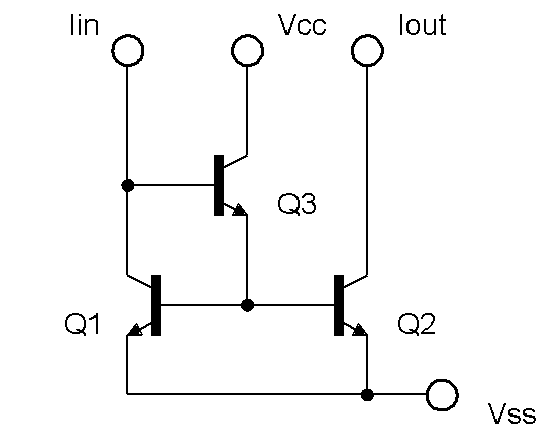
\includegraphics[scale=0.5]{obrazky/ZlepseneWilsonovoZrcadloNPN}
    \end{center}
    \caption[Alenčino zrcadlo]{Zlepšené Wilsonovo proudové zrcadlo.}
  \end{figure}

Pro odlišení tlačítek je místo označeno barevným potiskem. 

\section{Vibrační motor}
Vibrační motory jsou založeny na principu kmitání. Motor je připevněn k zařízení, které je kmitáním rozvibrováno. Vibrační motory jsou dnes 
nedílnou součástí mnoha elektronických zařízení včetně mobilního telefonu nebo dětských hraček. 

Dioda slouží jako ochrana proti přepětí, protože motor je indukční zátěž, takže vytváří napěťové špičky. Díky diodě je mikrokonrolér chráněn 
proti špičkovému napětí, které by se na něj mohlo dostat. Kondenzátor slouží k tomu, aby napěťové špičky eliminovat, nebo alespoň zmenšoval. 

Vibrační motor je připojen k mikrokontroléru přes tranzistor, protože maximální výstupní proud z pinu MCU není dostatečně velký na to, aby 
motor roztočil. Tranzistor je tedy připojen na gate tranzistoru, který se při logické jedničce na pinu sepne a motorem protéká proud, který 
nedodává MCU, ale zdroj 3.3 V (v tomto případě baterie LiFePO4). Baterie tak dokáže dodat dostatek proudu, aby se motor roztočil. 

Pro Semafor byl vybrán vibrační motor LCM1020A2945F. Tento motor má maximální požadovaný proud 120 mA \cite{vib_motor_dtsh}. Maximální proud, 
který lze odebírat z pinu mikrokontroléru ESP32-C3, je 40 mA \cite{ESP_C3_dtsh}. Vibrační motor lze pouze spínat, nebo je možné jej připojit 
k pinu, který dokáže generovat PWM a lze tím regulovat jeho otáčky. 

Vibrační motor slouží jako odezva na dotyk kapacitního tlačítka. 

%obrázek schéma zapojení + asi fotka vybraného motoru

\section{Převodník pro kapacitní tlačítka}
Vybraný mikrokonrolér ESP32-C3 nemá kapacitní vstupy, proto je zapotřebí kapacitní dotyková tlačítka připojit přes převodník. Je zapotřebí připojit 
5 tlačítek. 
%jaké byly možnosti 
%zmínit se i o TTP224?
%má 4 vstupy, ale já potřebuji 5 tlačítek

Použitý převodník AT42QT1070 dokáže pracovat ve 2 režimech. V prvním režimu může být zapojeno maximálně 5 kapacitních tlačítek, která jsou připojena
k pinům KEY0 až KEY4. Jako výstup se používají piny OUT0 až OUT4. Každé tlačítko má tedy svůj výstup, který může být připojen k GPIO pinům MCU 
nebo k nim mohou být připojeny např. LED \cite{conv_cap_but_AT42QT1070_dtsh}. 

Druhý režim je využitelný pouze v případě, je-li převodník připojen k MCU. Vtomto případě může být k převodníku připojeno až 7 kapacitních tlačítek, 
která jsou připojena na pinech KEY0 až KEY6. Převodník poté komunikuje s MCU pomocí komunikační sběrnice I2C \cite{conv_cap_but_AT42QT1070_dtsh}. 
Z registru převodníku lze poté vyčíst stavy daných kapacitních dotykových tlačítek. 

Jelikož je v tomto návrhu Semaforu využit mikrokontrolér, který podporuje komunikaci po sběrnici I2C, tak bylo využito právě zapojení s komunikací 
přes I2C. Díky tomu budou využity pouze 2 GPIO piny mikrokonroléru ESP32-C3 a ne 5 GPIO pinů, které by byly zapotřebí při zapojení bez komunikace pro
sběrnici I2C.

Převodník má kondenzátory C3 a C4 připojeny na napájecím pinu vůči zemi, aby nebyly případné proudové špičky přivedeny na napájení převodníku. Rezistory
R17 a R18 slouží jako pull-up rezistory při komunikaci pomocí sběrnice I2C s mikrokonrolérem EP32-C3. Na piny KEY0 až KEY4 jsou připojena kapacitní 
dotyková tlačítka.  
%proč je MODE na zemi
%proč nepoužívám pin /CHANGE?
%obrázek - schéma


\section{Baterie}
Ve výběru baterií hraje velkou roli kapacita, napětí, velikost a cena. Požadavkem je také možnost nabíjení, protože není žádoucí, aby si uživatel
baterie měnil. Při použití na táboře by také musely být stále nové baterie v balení a musely by se neustále doplňovat a udržovat.

Vybraný mikrokonrolér má napájecí napětí v rozsahu 3 až 3,6 V \cite{ESP_C3_dtsh}. 

Z nabíjecích baterií je možno vybírat z nabíjecích tužkových baterií (Ni-MH), Li-Ion, Li-Pol a LiFePO4 baterií.
%Ni-MH
Baterie Ni-MH mají jmenovité napětí 1,25 V. %citace
Proto by bylo zapotřebí alespoň 3 článků spojených sériově, u kterých by navíc musel být stabilizátor
na 3,3 V pro napájení mikrokontroléru. % a co inteligentní LED?
%Li-Ion

%Li-Pol

%LiFePO4
LiFePO4 baterie mají jmenovité napětí v rozsahu %xyz V + citace.



\section{Nabíjecí obvod}
Nabíjecí obvody jsou závislé na konkrétním typu baterií, které budou nabíjeny. Vzhledem k vybranému typu baterií LiFePO4 byly uvažovány pouze komerčně
dostupné integrované obvody, které jsou určeny pro nabíjení tohoto typu baterií. 

Vybraný typ baterií LiFePO4 lze nabíjet pomocí obvodu CN3058E \cite{charger_dtsh}. 
%možná vyjmenovat další obvody a napsat proč tento

Nabíjecí obvod CN3058E je určen pro nabíjení pouze LiFePO4 baterií a lze jím napájet právě 1 článek těchto baterií \cite{charger_dtsh}. Napájecí napětí tohoto 
nabíjecího čipu se pohybuje mezi 3,8 až 6 V \cite{charger_dtsh}. Díky tomu lze použít, bez jakéhokoli napěťového převodníku, napájení z USB konektoru. 

%popsat další vlastnosti 

%doporučené schéma zapojení čipu - z datasheetu

Tento nabíjecí obvod se vyrábí ve standardizovaném pouzdře SOP8 \cite{charger_dtsh}.

\subsection{Zapojení nabíjecího obvodu}
Rezistor připojený k pinu ISET slouží pro nastavení hodnoty nabíjecího proudu \cite{charger_dtsh}. V tomto zapojení byl počítán pro nabíjecí proud 1 A. 

%1218/1 = 1218 Ohm
%rovnici + citace

Z výpočtu vyplývá, že rezistor by měl mít hodnotu 1218 $\Omega$. Nejbližší hodnota z rezistorové řady E12 je hodnota 1,2 k$\Omega$, proto byl také zvolen rezistor 
o této hodnotě \cite{rezistorova_rada}. Odpovídá tomu nabíjecí proud 1015 mA, který nebude mít vliv na životnost baterií. 

%rovnice 1218/1200 = 1.015 A = 1015 mA

Vstupní a výstupní kondenzátory slouží pro filtaci zákmitů napájecího napětí a také napětí, kterým je nabíjena baterie. Hodnoty kondenzátorů byly převzaty
z doporučení z datasheetu.

Kladný pól nabíjené baterie je připojen na pinu BAT, záporný pól je připojen ke GND. 
%do zkratek přidat GND

Tento nabíjecí obvod má možnost indikace nabíjení baterií a dokončení nabíjení. Tato indikace je realizována pomocí 2 LED připojených přes pull-up rezistor. Hodnota
pull-up rezistoru byla převzata z doporučení z datasheetu. Červená LED indikuje nabíjení baterií a je připojena na pin /CHRG a zelená LED indikuje dokončené nabíjení 
a je připojena na pin /DONE. Obě LED jsou k pinům nabíjecího čipu připojeny katodou. 

Obvod CN3058E může také měřit teplotu na nabíjené baterii. Slouží k tomu pin TEMP. Měření probíhá pomocí odporového děliče, jehož střed je připojen na snímač teploty. 
Tento snímač je připojen na baterii. V této práci není měření teploty baterií využíváno, a proto není pin obvodu TEMP nikam připojen. 

%obrázek z datasheetu, kde je připojeno i meření teploty

Pokud není baterie nabíjena, tak by svodový proud pinu BAT nabíjecího obvodu CN3058E vibíjel baterii. Svodový proud tohoto pinu je 3 $\mu$A \cite{charger_dtsh}. 
Aby se baterie zbytečné navybíjela, tak je do obvodu připojen tranzistor Q2, který detekuje připojené napětí k nabíjecímu obvodu. Pokud je napětí připojeno, tak je 
tranzistor otevřen a baterie je nabíjena. Pokud napětí připojeno není, tak je tranzistor uzavřen a baterie je díky tomu odpojena od nabíjecího obodu. Díky tomu 
není vybíjena svodovým proudem pinu BAT. 

\section{Zvyšovač napětí pro LED}
Pro napájení vybraných inteligentních LED je zapotřebí napětí v rozsahu %xxx V proč chci vyrábět právě 5?

Z komerčně dostupných integrovaných obvodů byl hledán zvyšovač napětí, který zvládne z 3,3 V vytvořit napětí 5 V a dodávat přitom alespoň 200 mA. %proč 180 mA
Vyhovující těmto parametrům byly nalezeny obvody LT1930 a MCP1640. 

%schéma zapojení z datasheetu

Obvod LT1930 v doporučeném zapojení při vstupním napětí 3,3V vytváří výstupnní napětí o hodnotě 5 V s maximálním odběrem proudu 480 mA \cite{LT1930_dtsh}. Napájecí napětí 
tohoto obvodu je v rozsahu 2,45 až 16 V, což vyhovuje napájecímu napětí z baterií LiFePO4 \cite{LT1930_dtsh}.
%rozsah výstupního napětí
%další důležité parametry

Pin /SHDN slouží k zapínání a vypínání obvodu. Pomocí přiloženého napětí 2,4 V a více na tento pin je obvod zapnut \cite{LT1930_dtsh}. Pin SW slouží pro  připojení cívky, 
případně diody, aby se snížilo elektromagnetické rušení \cite{LT1930_dtsh}. Pin FB slouží  pro zapojení zpětné vazby. Jeho referenční napětí je 1,255 V \cite{LT1930_dtsh}. 
Slouží pro připojení odbočky z odporového děliče, díky čemuž je nastaveno výstupní napětí \cite{LT1930_dtsh}.
%napsat vzorec jako rovnici V OUT = 1.255V(1 + R1/R2) a odcitovat

%zvyšovač napětí z 3V3 na 5V
% vzorec pro výpočet odporů

%proč byl vybrán právě tento?

%výběr diody
%výběr cívky
%schéma zapojení vybraného typu

\section{Konektor}
Jako nabíjecí a zároveň programovací konektor byl zvolen konektor USB typu C.

Tento konektor je v dnešní době velmi rozšířený a jeho použití se v následující době stále rozšiřuje. 

Není využíváno žádných výhod konektoru USB-C, jako je např. možnost power delivery apod. Je využíván pouze jako standardní a dostupný konektor, který je mezi běžnou
populací rozšířený a v následujících letech se bude rozšiřovat stále více. Je využito standardního jmenovitého napětí 5 V pro nabíjení baterií a nadále pinů D+ a D-, 
které jsou využity pro komunikaci při programování. 

Konektor USB-C je robustní a oboustranný, díky čemuž nebude docházet k tak častému poškození, jak by mohlo být např. u konektoru Micro USB. Při používání běžnou veřejností
se jedná o vítaný bonus. čš

Vybraný mikrokonrolér ESP32-C3 umožňuje komunikaci přímo po USB protokolu a není díky tomu zapotřebí žádného převodníku pro komunikaci \cite{ESP_C3_dtsh}. %jmenuje se to USB protokol?

%o transilech k USB + Shotkyny
%o rezistorech 5,1k

%na konci bude muset být blokové schéma konkrétních (vybraných) modulů

%popsat převodník komunikačních úrovní pro LED a Mikrokontrolér

%power led pro první prototyp, potom nebudou, kvůli šetření energie, protože je to na baterky a mohlo by to při hrách hráče mást

%zvukova sinalizace - piezo


%%% Vložení souboru 'text/vysledky' s popisem vysledků práce
% (rozdělte na více souborů či kapitol, pokud je vhodné)
\chapter{Výběr a návrh elektroniky}
Výběr elektronických součástek probíhal dle jejich parametrů, využití, dostupnosti a~ceny. Nejdříve byla vybrána bezdrátová technologie a mikrokontrolér a v~závislosti 
na tom vše ostatní. 

\section{Bezdrátová technologie}
Ke komunikaci Univerzálních modulů mezi sebou byla zvolena technologie LoRa a pro bezdrátovou konfiguraci Univerzálních modulů byla zvolena technologie WiFi. 

\subsection{WiFi}
Pro bezdrátovou konfiguraci byla vybrána WiFi technologie, protože ji má k dispozici každý ve svém telefonu a notebooku. Zároveň ji každý laik umí základně ovládát. Jedná se 
o~rozšířenou technologii. 
Propojení bude tedy jednoduché a nastavování her může probíhat na webové stránce, kde bude seznam her, které Univerzální modul umí. U~jednotlivých her se poté budou moci nastavovat 
další parametry. Po nastavení se konfigurace pošle právě pomocí WiFi do Univerzálního modulu. Některé mikrokontroléry mají WiFi zabudovanou, takže jedním z kritérií pro výběr 
mikrokontroléru se stala právě WiFi, která musí být jeho součástí. 

\subsection{LoRa}
Tato technologie byla zvolena především pro možnost rozšíření využití Univerzálního modulu. Pro toto využití byla vybrána technologie LoRa především kvůli komunikačnímu dosahu. 
Může být využita pro komunikaci Univerzálních modulů mezi sebou. Mohou si tak předávat informace například o aktuálně svítící barvě nebo o stisknutých tlačítkách. Využití je
závislé na konkrétní aktivitě. U některých her může být například žádoucí, aby po přepínání nesvítily všechny Univerzální moduly stejnou barvou a díky této komunikaci bude moci 
být takovým stavům zabráněno. Jedná se sice o~dražší technologii, 
ale ne na tolik, aby ji nebylo možné v~tomto zařízení použít. Outdoorové aktivity se většinou odehrávají na prostranství, která mají velkou rozlohu. LoRa je jedinou
dostupnou technologií, která na velké vzdálenosti spolehlivě komunikuje.  

Byl vybrán bezdrátový LoRa modul E22-900T22D od firmy EBYTE. Tento modul komunikuje s mikrokontrolérem pomocí UART sběrnice \cite{LoRa_ebyte}. Jeho napájecí napětí je od 
2,1 V do 5,5 V a komunikační napětí je 3,3 V \cite{LoRa_ebyte}. Rozsah komunikačních frekvencí bezdrátového modulu E22-900T22D je 850,125 MHz až 930,125 MHz a ve výchozím 
stavu je nastavena na 868,125 MHz \cite{LoRa_ebyte}. Toto je frekvence, na které je v ČR povoleno komunikovat a to s maximálním vyzařovaným výkonem 25 mW \cite{CTU}. 
Maximální povolený klíčovací poměr je 1 \% \cite{CTU}. %klíčovací poměr = max duty cycle 
V běžném režimu je spotřeba přibližně 151 mA a v režimu spánku 2 $\mu$A \cite{LoRa_ebyte}. Tento bezdrátový modul má externě připojitelnou anténu typu SMA-K s 50 $\Omega$ 
impedancí \cite{LoRa_ebyte}.

LoRa modul E22-900T22D je připojen k mikrokontroléru pomocí komunikačních pinů RX a TX sběrnice UART. Napájecí napětí tohoto modulu je spínáno mikrokontrolérem, aby jej 
šlo v případě nůzkého napětí baterie odpojit. Pin AUX slouží k indikaci funkčního stavu modulu. Při specifických aplikacích slouží pro probuzení externího mikrokontroléru. 
Pin AUX není v této aplikaci využíván, a proto není nikam připojen. Pomocí pinů M0 a M1 lze přepínat bezdrátový modul do různých režimů. Pokud jsou oba piny v logické 1, 
tak je modul přepnut do režimu spánku \cite{LoRa_ebyte}. Pokud jsou oba piny v logické 0, tak je modul v normálním režimu \cite{LoRa_ebyte}. V této aplikaci je modul 
provozován pouze v normálním režimu, a proto jsou piny M0 a M1 připojeny k signálu GND. 

\begin{table}[!h]
  \caption[Konfigurační piny LoRa modulu E22-900T22D]{Konfigurační piny LoRa modulu E22-900T22D \cite{LoRa_ebyte}}
  \begin{center}
  	\small
	  \begin{tabular}{|c|c|c|c|}
	    \hline
	    \textbf{M0}	& \textbf{M1}	& \textbf{Mód} & \textbf{Popis} \\
	    \hline
	    0	& 0 & Normální & UART a bezdrátový kanál otevřený, \\ 
      & & &transparentní přenos zapnutý \\ 
	    \hline
	    0	& 1 & Režim WOR & Lze definovat jako vysílač WOR \\
      & & & a přijímač WOR \\ 
	    \hline
	    1 & 0 & Konfigurační mód & Přistup k registru přes sériový port \\
      & & & a ovládání pacovního stavu \\
	    \hline
      1 & 1 & Režim hlubokého & Režim spánku \\
      & & spánku & \\
	    \hline
	  \end{tabular}
  \end{center}
\end{table}

%obrazek se zapojenim LoRa modulu

\section{Mikrokontrolér}
WiFi modul obsahují mikrokontroléry od firmy Espressif z~řady ESP32. Vybrán byl typ ESP32-C3-MINI-1, dále již jen ESP32-C3. Tento mikrokontrolér je nabízen za cenu, která 
je v~porovnání s~ostatními nízká a v~porovnání s~nabízenými parametry bezkonkurenční. Pro zařízení Univerzálního modulu je také se svým počtem periferií dostačující. ESP32-C3 má 
384 kB ROM a 4 MB flash paměti \cite{ESP_C3_dtsh}. Dále obsahuje WiFi modul pracující na frekvenci 2,4 GHz a Bluetooth \cite{ESP_C3_dtsh}. ESP32-C3 obsahuje mnoho periferií
jako je SPI, UART, $I^2C$, USB a další \cite{ESP_C3_dtsh}. Mikrokontrolér má vyvedeno 13 GPIO pinů, které je možno softwarově nastavit jako vstupní nebo výstupní. Tyto piny
slouží pro připojení senzorů, díky kterým je zprostředkována komunikace mezi mikrokontrolérem a okolním prostředím. Na pinech GPIO0, GPIO1, GPIO2, GPIO3, GPIO4 a GPIO5 jsou 
k dispozici AD převodníky \cite{ESP_C3_tech_ref}. V~mikrokontroléru je také zabudován krystal s~vlastní frekvencí 
40 MHz a v~rámci pouzdra je také anténa pro WiFi \cite{ESP_C3_dtsh}.

\begin{figure}[!h]
  \begin{center}
    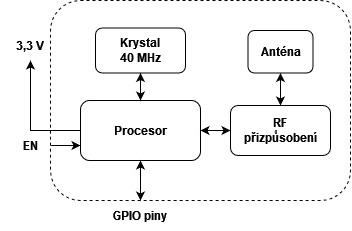
\includegraphics[scale=0.8]{obrazky/blokove_schema_MCU.jpg}
  \end{center}
  \caption[Blokové schéma mikrokontroléru ESP32-C3]{Blokové schéma mikrokontroléru ESP32-C3 \cite{ESP_C3_dtsh}.}
\end{figure}

Rozsah napájecího napětí je 3~až 3,6~V~\cite{ESP_C3_dtsh}. Jeho maximální proudový odběr je 0,5~A~\cite{ESP_C3_dtsh}. Mikrokontrolér ESP32-C3 garantuje pracovní teplotu 
od -45~°C až do 85~°C \cite{ESP_C3_dtsh}.

K~pinu 3V3, který slouží pro připojení napájecího napětí, je připojeno bateriové napětí, a také jsou k němu připojeny kondenzátory o~hodnotě 10 $\mu$F a 100 nF dle doporučení z~dokumentace \cite{ESP_C3_dtsh}. Tyto 
kondenzátory slouží pro filtraci napájecího napětí, aby bylo vyfiltrováno případné rušení o~různých frekvencích.

Pin EN slouží pro povolení funkce mikrokontroléru. Tento pin nesmí zůstat nezapojený, tzv. floating. Jeho zapojení je převzato z~dokumentace, tj. pullup rezistor o~hodnotě 
10 k$\Omega$ a ke GND je připojen přes kondenzátor o~hodnotě 1 $\mu$F \cite{ESP_C3_dtsh}.

ESP32-C3 má konfigurační piny, které slouží při restartu pro určení, odkud bude načten program pro mikrokontrolér. Tyto piny musí být při restartu v~daném nastavení. 
Konfiguračními piny jsou GPIO2, GPIO8 a GPIO9. Piny GPIO8 a GPIO9 nesmí být nikdy nastaveny současně do logické nuly. 

\begin{table}[!h]
  \caption[Konfigurační piny ESP32-C3]{Konfigurační piny ESP32-C3 \cite{ESP_C3_dtsh}}
  \begin{center}
  	\small
	  \begin{tabular}{|c|c|c|c|}
	    \hline
	    \textbf{Pin}	& \textbf{Výchozí}	& \textbf{Načtení programu} & \textbf{Načtení programu} \\
      \textbf{}	& \textbf{}	& \textbf{z~flash paměti} & \textbf{z~bootloaderu} \\
	    \hline
	    \textbf{GPIO2}	& Není dostupný & 1 & 1 \\ 
	    \hline
	    \textbf{GPIO8}	& Není dostupný & Nezáleží & 1 \\ 
	    \hline
	    \textbf{GPIO9} & Interní měkký pullup & 1 & 0 \\
	    \hline
	  \end{tabular}
  \end{center}
\end{table}

Protože bude využito programování přes USB piny D+ a D-, tak není zapotřebí načtení z~bootloaderu a je tedy zapotřebí všechny konfigurační piny při restartu připojit do 
logické jedničky. Do logické jedničky lze připojit přes pullup rezistor. Pullup rezistory má sběrnice $I^2C$, takže na GPIO8 a GPIO9 byla připojena právě sběrnice $I^2C$.
Pin GPIO2 nebyl využit pro připojení žádného senzoru, a proto byl připojen přes pullup rezistor o~hodnotě 10 k$\Omega$ k~napájecímu napětí.

Na pin GPIO4 je připojeno měření napětí na baterii. Na tomto pinu je k dispozici AD převodník s nastavitelnou hodnotou referenčního napětí \cite{ESP_C3_tech_ref}. Hodnota 
rezistorového děliče byla tedy přizpůsobena tomuto rozsahu možného měřeného napětí. 

\begin{figure}[!h]
  \begin{center}
    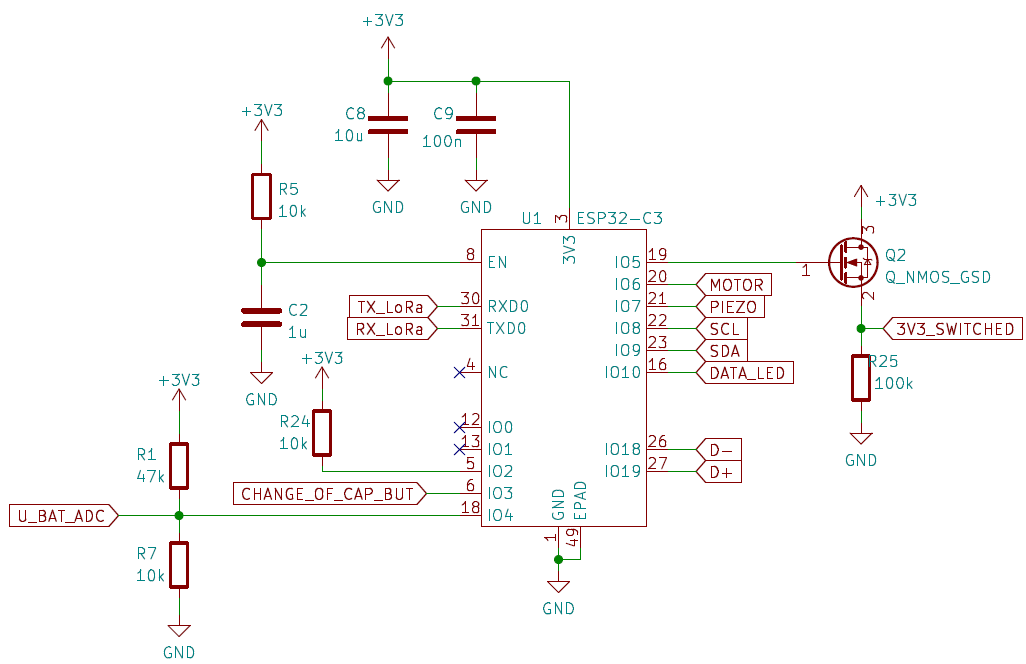
\includegraphics[scale=0.5]{obrazky/ESP32-C3.png}
  \end{center}
  \caption[Schéma zapojení mikrokontroléru ESP32-C3]{Schéma zapojení mikrokontroléru ESP32-C3.}
\end{figure}

Na piny GPIO18 a GPIO19 je možné připojení pinů D+ a D-, takže USB piny byly připojeny k mikrokontroléru napřímo bez použití jakéhokoli převodníku \cite{ESP_C3_dtsh}. Díky 
tomu také mohou být piny sériové linky RX a TX využity pro připojení LoRa modulu E22-900T22D.

K pinu GPIO5 je připojen PMOS tranzistor, který spíná napájecí napětí některým periferiím, které mají vyšší spotřebu. Napájecí napětí tak může být odpojováno například v době,
kdy je na baterii nízké napětí. Provozní doba Univerzálního modulu se tak proudlouží a nedojde tak k podvybití baterie a k jejímu možnému následnému poškození. 

\section{Napájení}
Zabudování baterie přináší kompaktnost řešení a pro použití není třeba dalších komponent. Pokud je ale na táboře větší využití, tak se baterie vybije.
Na táborech většinou nebývá k~dispozici připojení k~elektrické síti, a proto je řešením powerbanka. Na Univerzálním modulu tedy bude napájecí vstup USB-A pro nabíjení 
baterií přímo z~powerbanky bez nutnosti kabelu. Univerzální modul musí být koncipován tak, aby se mohla baterie nabíjet a zároveň, aby při tom byly Univerzální moduly 
funkční.

Při realizaci Univerzálního modulu byla tedy zvolena kombinace napájení pomocí baterií i~pomocí powerbanky. Článek baterie LiFePO4 byl vybrán právě kvůli již zmíněným 
vynikajícím vlastnostem. Vybraný mikrokontrolér má napájecí napětí v~rozsahu 3 až 3,6 V~\cite{ESP_C3_dtsh}. Pro funkci mikrokontroléru tedy nebude muset být použit ani 
převodník napětí. 

Napětí na baterii je měřeno pomocí děliče a připojeno na pin GPIO4, který má k~dispozici AD převodník \cite{ESP_C3_dtsh}. V~softwaru bude nastaven útlum na 0 dB, to 
odpovídá rozsahu měřeného napětí od 0 do 700 mV \cite{ESP_C3_tech_ref}.
Proto je napětí z~baterie pomocí rezistorového děliče převedeno na rozsah od 0 do 600 mV. Zde je pomocí AD převodníku napětí na baterii měřeno. Spodní rezistor děliče byl
zvolen o~hodnotě 10 k$\Omega$ a druhý byl dopočítán na hodnotu 50 k$\Omega$ podle maximálního napětí baterií LiFePO4, tj. 3,6 V. Nejbližší hodnota rezistoru je 47 k$\Omega$
\cite{rezistorova_rada}. Tomu odpovídá maximální napětí na AD převodníku 0,63 V, což je stále v~možném měřeném rozsahu. 

%tuhle větu upravit - přesunout někam 
Při nízkém napětí baterie je díky měření možno softwarově zareagovat. Lze například odpojit napájecí napětí některým periferiím s vyšší spotřebou.

\subsection{Nabíjecí obvod}
Nabíjecí obvody jsou závislé na konkrétním typu baterií, které budou nabíjeny. Vzhledem k~vybranému typu baterií LiFePO4 byly uvažovány pouze komerčně
dostupné integrované obvody, které jsou určeny pro nabíjení tohoto typu baterií. 

Vybraný typ baterií LiFePO4 lze nabíjet pomocí obvodu CN3058E. 

Nabíjecí obvod CN3058E je určen pro nabíjení pouze LiFePO4 baterií a lze jím napájet právě 1 článek těchto baterií \cite{charger_dtsh}. Napájecí napětí tohoto 
nabíjecího čipu se pohybuje mezi 3,8 až 6 V~\cite{charger_dtsh}. Díky tomu lze přímo použít napětí z~USB konektoru. 

Když je nabíjecí obvod odpojen od napájecího napětí, tak přejde do režimu spánku \cite{charger_dtsh}. V~tomto režimu je baterie vybíjena proudem menším než 
3 $\mu$A \cite{charger_dtsh}. Tento proud je oproti klidovým proudům jiných součástek zanedbatelný, a proto nemusí být baterie od nabíjecího obvodu odpojována,
když není nabíjena. 

Nabíjecí obvod CN3058E umí také vyhodnocovat teplotu baterie a v~závislosti na tom přestávat baterii nabíjet \cite{charger_dtsh}. Tato funkce není v~zapojení
Univerzálního modulu využita, proto je pin TEMP připojen k~signálu GND \cite{charger_dtsh}.

Tento nabíjecí obvod se vyrábí ve standardizovaném pouzdře SOP8 \cite{charger_dtsh}.

\subsection{Zapojení nabíjecího obvodu}
Rezistor připojený k~pinu ISET slouží pro nastavení hodnoty nabíjecího proudu \cite{charger_dtsh}. V~tomto zapojení byl počítán pro nabíjecí proud 1 A~dle rovnice
z~dokumentace: 
\begin{equation} 
  R_{8}~=~\frac{1218}{I_{CH}}~=~\frac{1218}{1}~=~1,218~k\Omega. 
  \quad \quad \quad \quad \quad \quad \quad \quad \quad \cite{charger_dtsh}
\label{eq:I_CH}
\end{equation}

Z~výpočtu vyplývá, že rezistor by měl mít hodnotu 1,218 k$\Omega$. Nejbližší hodnota z~rezistorové řady E12 je hodnota 1,2 k$\Omega$, proto byl také zvolen rezistor 
o~této hodnotě \cite{rezistorova_rada}. Odpovídá tomu nabíjecí proud 1015 mA, který nebude mít vliv na životnost baterií. 

Vstupní a výstupní kondenzátory slouží pro filtraci zákmitů napájecího napětí a také napětí, kterým je nabíjena baterie. Hodnoty kondenzátorů byly převzaty
z~doporučení z~dokumentace, tj. 4,7 $\mu$F \cite{charger_dtsh}.

Kladný pól nabíjené baterie je připojen na pinu BAT, záporný pól je připojen ke GND. Pin BAT poskytuje nabíjecí proud do baterie a zároveň poskytuje konstantní 
nabíjecí napětí. V~režimu spánku je svodový proud tohoto pinu 3 $\mu$A \cite{charger_dtsh}. 

Pin VIN slouží pro napájení vnitřního obvodu CN3058E. Je na něj přikládáno napájecí napětí z~USB, tedy 5 V. Pokud napájecí napětí klesne na napětí o~10 mV nižší, 
než je napětí na pinu BAT, tak vnitřní obvod přechází do režimu spánku \cite{charger_dtsh}. V~tomto režimu klesá proud pinu BAT na méně než 3 $\mu$A \cite{charger_dtsh}.

Tento nabíjecí obvod má možnost indikace nabíjení baterií a dokončení nabíjení. Tato indikace je realizována pomocí 2 LED připojených přes pullup rezistor. Hodnota
pullup rezistoru byla převzata z~doporučení z~dokumentace, tj. 330 $\Omega$. Červená LED indikuje nabíjení baterií a je připojena na pin /CHRG a zelená LED indikuje 
dokončené nabíjení a je připojena na pin /DONE. Obě LED jsou k~pinům nabíjecího čipu připojeny katodou. 

Obvod CN3058E může také měřit teplotu na nabíjené baterii. Slouží k~tomu vstupní pin TEMP. Měření probíhá pomocí odporového děliče, jehož střed je připojen na snímač 
teploty. Tento snímač je připojen na baterii. Pokud je napětí na pinu TEMP nižší než 45 \% nebo vyšší než 80 \% úrovně napájecího napětí, tak je indikována moc nízká
nebo moc vysoká teplota baterie a nabíjení je zastaveno \cite{charger_dtsh}. Jinak nabíjení pokračuje. Uzemněním pinu TEMP je funkce měření teploty deaktivována 
\cite{charger_dtsh}. V~této práci není měření teploty baterií využíváno, a proto je pin TEMP připojen ke GND. 

\begin{figure}[!h]
  \begin{center}
    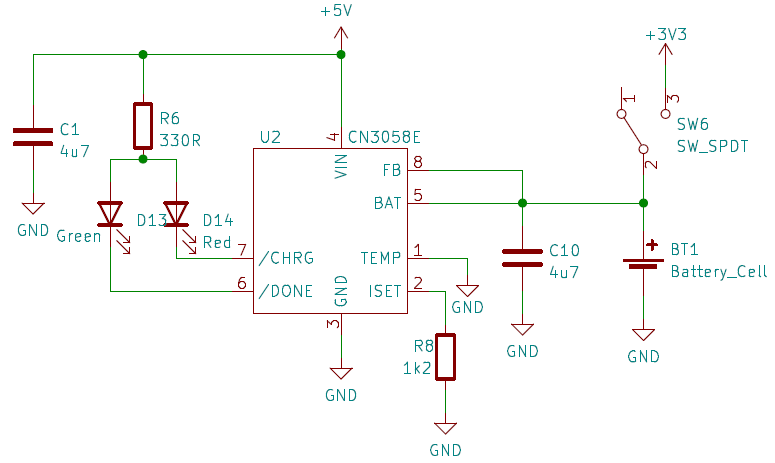
\includegraphics[scale=0.6]{obrazky/CN3058E.png}
  \end{center}
  \caption[Schéma zapojení nabíjecího obvodu pro LiFePO4]{Schéma zapojení nabíjecího obvodu pro LiFePO4.}
\end{figure}

\section{Senzory doteku}
V~návrhu Univerzálního modulu byla zvolena kapacitní dotyková tlačítka. Pro možnost použití uvnitř i venku jsou díky možnosti voděodolnosti 
vhodnějším řešením. Také velikost a označení tlačítka je variabilnější. Velikost může být na DPS navržena dle potřeby a potisk
v~místě tlačítka vyznačen barevně, nebo označen např. samolepkou. Odezva na dotyk bude realizována pomocí vibračního motoru.

\section{Vibrační motor}
Vibrační motory jsou založeny na principu kmitání. Motor je připevněn k~zařízení, které je kmitáním rozvibrováno. Vibrační motory jsou dnes 
nedílnou součástí mnoha elektronických zařízení včetně mobilního telefonu nebo dětských hraček. 

Dioda slouží jako ochrana proti přepětí, protože motor je indukční zátěž, takže vytváří napěťové špičky. Díky diodě je mikrokontrolér chráněn 
proti špičkovému napětí, které by se na něj mohlo dostat. Kondenzátor slouží k~tomu, aby napěťové špičky eliminoval, nebo alespoň zmenšoval. 

Vibrační motor je připojen k~mikrokontroléru přes tranzistor, protože maximální výstupní proud z~pinu MCU není dostatečně velký na to, aby 
motor roztočil. Tranzistor je tedy připojen na gate tranzistoru, který se při logické jedničce na pinu sepne a motorem protéká proud, který 
nedodává MCU, ale zdroj 3.3 V~(v~tomto případě baterie LiFePO4). Baterie tak dokáže dodat dostatek proudu, aby se motor roztočil. 

Pro Univerzální modul byl vybrán vibrační motor LCM1020A2945F. Tento motor má maximální požadovaný proud 120 mA \cite{vib_motor_dtsh}. Maximální 
proud, který lze odebírat z~pinu mikrokontroléru ESP32-C3, je 40 mA \cite{ESP_C3_dtsh}. Vibrační motor lze pouze spínat, nebo je možné jej připojit 
k~pinu, který dokáže generovat PWM a lze tím regulovat jeho otáčky. 

Vibrační motor slouží jako odezva na dotyk kapacitního tlačítka. 

\begin{figure}[!h]
  \begin{center}
    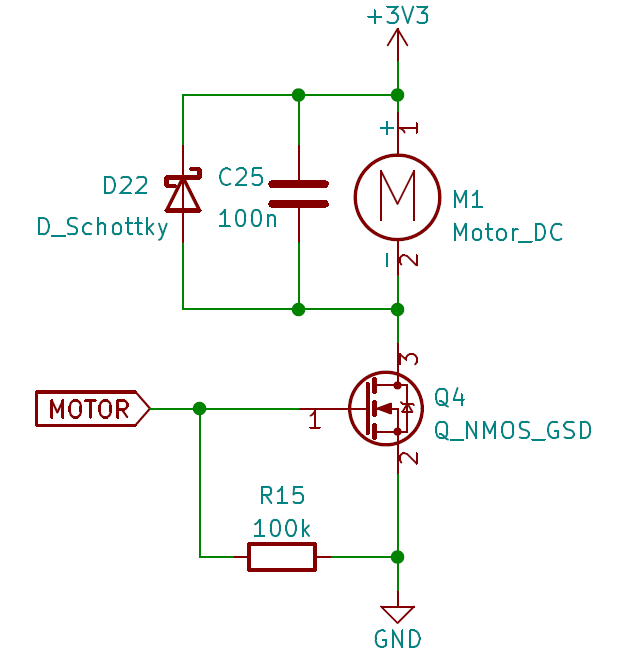
\includegraphics[scale=0.4]{obrazky/Vibracni_motor.png}
  \end{center}
  \caption[Schéma zapojení vibračního motoru]{Schéma zapojení vibračního motoru.}
\end{figure}

%fotka vybraného motoru

\section{Převodník pro kapacitní tlačítka}
Mikrokontrolér ESP32-C3 nemá kapacitní vstupy, proto je zapotřebí kapacitní dotyková tlačítka připojit přes převodník. Je zapotřebí připojit 
5 tlačítek. 

Vybraný převodník AT42QT1070 dokáže pracovat ve 2 režimech. V~prvním režimu může být zapojeno maximálně 5 kapacitních tlačítek, která jsou připojena
k~pinům KEY0 až KEY4. Jako výstup se používají piny OUT0 až OUT4. Každé tlačítko má tedy svůj výstup, který může být připojen k~GPIO pinům MCU 
nebo k~nim mohou být připojeny např. LED \cite{conv_cap_but_AT42QT1070_dtsh}. 

Druhý režim je využitelný pouze v~případě, je-li převodník připojen k~MCU. V~tomto případě může být k~převodníku připojeno až 7 kapacitních tlačítek, 
která jsou připojena na pinech KEY0 až KEY6. Převodník poté komunikuje s~MCU pomocí komunikační sběrnice $I^2C$ \cite{conv_cap_but_AT42QT1070_dtsh}. 
Z~registru převodníku lze poté vyčíst stavy daných kapacitních dotykových tlačítek. 

Jelikož je v~tomto návrhu Univerzálního modulu využit mikrokontrolér, který podporuje komunikaci po sběrnici $I^2C$, tak bylo využito zapojení právě s~tímto typem 
komunikace. Díky tomu budou využity pouze 2 GPIO piny mikrokontroléru ESP32-C3 a ne 5 GPIO pinů, které by byly zapotřebí při zapojení bez komunikace pro
sběrnici $I^2C$. Komunikační sběrnice $I^2C$ vyžaduje pullup rezistory, proto byly mezi napájecí napětí a piny SDA a SCL převodníku AT42QT1070 
přidány rezistory R17 a R18 o hodnotě 10 k$\Omega$. To znamená, že komunikační sběrnice $I^2C$ je aktivní v logické nule. 

Kapacitní tlačítka jsou připojena přes rezistory R19 až R23 k převodníku AT42QT1070. Tyto rezistory jsou připojeny sériově a slouží ke snížení šumu, 
omezení elektrostatických výbojů a potlačení radiofrekvenčního rušení \cite{conv_cap_but_AT42QT1070_dtsh}. Doporučená hodnota je rezistorů je mezi 
4,7k$\Omega$ a 20 k$\Omega$ \cite{conv_cap_but_AT42QT1070_dtsh}. Byla zvolena střední hodnota z doporučeného rozsahu, tj 10 k$\Omega$.

Převodník má kondenzátory C3 a C4 připojeny na napájecím pinu vůči GND, aby nebyly případné proudové špičky přivedeny na napájení převodníku. Rezistory
R17 a R18 slouží jako pullup rezistory při komunikaci pomocí sběrnice $I^2C$ s~mikrokontrolérem EP32-C3. Na piny KEY0 až KEY4 jsou připojena kapacitní 
dotyková tlačítka. 

\begin{figure}[!h]
  \begin{center}
    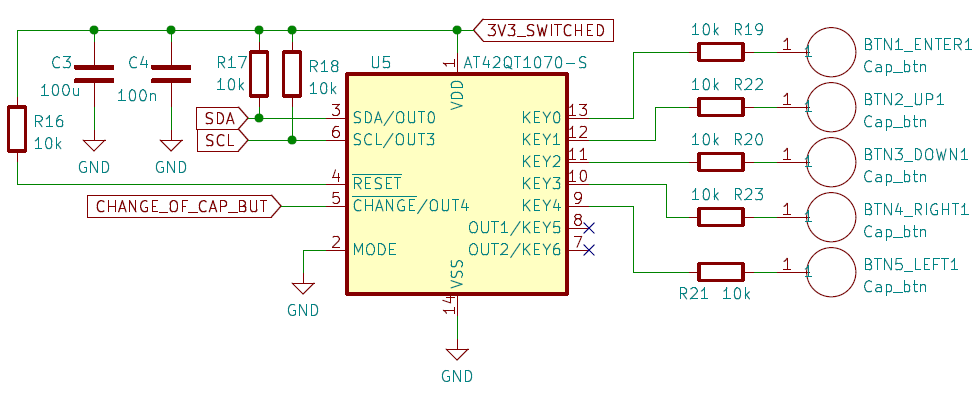
\includegraphics[scale=0.4]{obrazky/AT42QT1070.png}
  \end{center}
  \caption[Zapojení převodníku AT42QT1070 pro kapacitní tlačítka]{Zapojení převodníku AT42QT1070 pro kapacitní tlačítka.}
\end{figure}

Pin MODE je připojen k~signálu GND, protože převodník je provozován v~režimu komunikujícím přes $I^2C$ sběrnici \cite{conv_cap_but_AT42QT1070_dtsh}.

Pin /CHANGE je připojen k~GPIO pinu mikrokontroléru. Slouží pro indikaci změny stavu některého z~připojených tlačítek \cite{conv_cap_but_AT42QT1070_dtsh}. 
Signál z~tohoto pinu lze tedy využít jako indikátor vyvolání přerušení pro obsluhu tlačítek. 

Pin KEY0 může být také využit pro tzv. ochrannou zónu \cite{conv_cap_but_AT42QT1070_dtsh}. Tento kanál slouží pro zabránění falešným 
detekcím \cite{conv_cap_but_AT42QT1070_dtsh}. Tento pin je citlivější než ostatní \cite{conv_cap_but_AT42QT1070_dtsh}. Ochranná zóna by měla být také větší 
než použitá tlačítka. Této funkce nebylo do prototypu DPS využito. 

\section{Světelná signalizace}
Pro realizaci signalizace přítomnosti napájecího napětí byly vybrány neprogramovatelné LED. Zelené LED byly vybrány dvě, jedna pro 
indikaci přítomnosti napětí 5~V a druhá pro indikaci přítomnosti napětí 3,3 V~z~baterií. Tyto LED budou použity pouze na prototypu 
pro ulehčení oživování. Dále budou odstraněny kvůli šetření energie, protože jde o~bateriově napájené zařízení. Přítomnost svitu 
tzv. power LED by také mohla mást při hře nebo různých úkolech.

Pro realizaci světelné signalizace pro hry byly vybrány inteligentní programovatelné LED typu WS2812C. Bylo jich použito 12, protože 
z~dvanácti LED lze jednoduše zhotovit ciferník pro odpočítávání času a také je lze rozdělit na segmenty na třetiny nebo čtvrtiny. 

\begin{figure}[!h]
  \begin{center}
    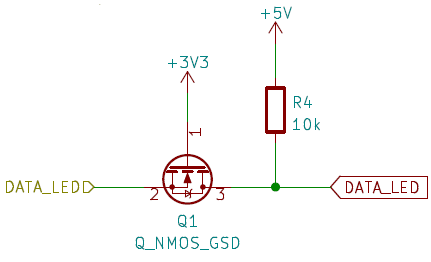
\includegraphics[scale=0.6]{obrazky/prevodnik_urovni_pro_WS2812C.png}
  \end{center}
  \caption[Zapojení převodníku úrovní pro WS2812C]{Zapojení převodníku úrovní pro WS2812C.}
\end{figure} 

Komunikační napěťová úroveň logické jedničky těchto LED by měla být alespoň na úrovni 70 \% napájecího napětí \cite{WS2812C_dtsh}. 
Protože použitý mikrokontrolér ESP32-C3 má komunikační napěťovou úroveň logické jedničky jeho napájecí napětí, což je 3 až 3,6 V, 
tak je zapotřebí využít převodník napěťové úrovně \cite{ESP_C3_dtsh}. Komunikace je v~tomto případě pouze jednosměrná, 
to znamená, že MCU posílá data do LED, ale LED neposílají žádná data do MCU. Převodník je realizován unipolárním tranzistorem 
a~jedním pullup rezistorem. Rezistor je připojen k~napájecímu napětí inteligentních LED WS2812C. 
Tranzistor Q1 má gate připojený k~napájecímu napětí MCU. Pokud bude mikrokontrolér do LED posílat logickou jedničku, tak bude rozdíl
mezi gate a~source 0 V. Tím pádem bude tranzistor uzavřený a tím se přes rezistor R4 připojí k~LED jejich napájecí napětí. Toto napětí 
je pro inteligentní LED logickou jedničkou. Pokud bude MCU posílat logickou nulu, tedy 0 V, tak je rozdíl napětí mezi gate a~source 
napájecí napětí mikrokontroléru. Tranzistor je tedy otevřený, a tím se napětí 0 V~dostane k~inteligentním LED a na rezistoru se objeví
úbytek napětí o~velikosti napájecího napětí inteligentních LED. Napětí 0 V~je logickou nulou i pro inteligentní LED. Tento převodník
je určen pouze pro komunikaci jedním směrem. 

\begin{figure}[!h]
  \begin{center}
    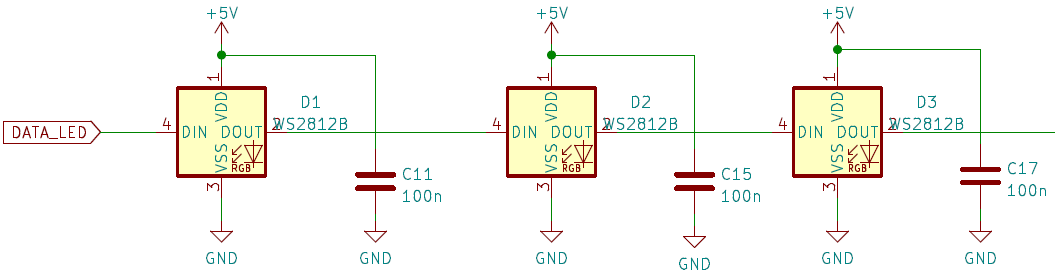
\includegraphics[scale=0.5]{obrazky/WS2812C.png}
  \end{center}
  \caption[Zapojení inteligentních LED WS2812C]{Zapojení inteligentních LED WS2812C.}
\end{figure}

Kondenzátor u~každé LED slouží pro filtraci napájecího napětí. 

Tyto programovatelné LED mají maximální spotřebu 5 mA na jeden kanál. Při zapnutí všech kanálů (svícení bílou) je maximální
spotřeba jedné LED 15 mA \cite{WS2812C_dtsh}. Pokud LED nesvítí, tak je její maximální klidový proud 0,3 mA \cite{WS2812C_dtsh}.
Při použití 12 LED je tedy maximální odběr všech LED 180 mA.

Pro napájení těchto inteligentních LED je zapotřebí napětí v~rozsahu 4,5 až 5,5~V \cite{WS2812C_dtsh}. 
Použité baterie LiFePO4 mají napětí pouze 3,2 V, proto je zapotřebí použít zvyšovač napětí na 5 V. 

\subsection{Zvyšovač napětí pro programovatelné LED}
Z~komerčně dostupných integrovaných obvodů byl hledán zvyšovač napětí, který vytváří z~napětí 3,3 V~napětí 5 V~a může přitom dodávat do výstupu proud alespoň 200 mA. 
Maximální odběr všech dvanácti potřebných inteligentní LED má maximální odběr 180 mA. S~rezervou je tedy zapotřebí proud alespoň 200 mA. Nalezené obvody, které vyhovují 
těmto parametrům jsou LT1930 a MCP1640. 

Obvod LT1930 v~doporučeném zapojení při vstupním napětí 3,3V vytváří výstupní napětí o~hodnotě 5 V~s~maximálním odběrem proudu 480 mA \cite{LT1930_dtsh}. Napájecí napětí 
tohoto obvodu je v~rozsahu 2,45 V~až 16 V, což vyhovuje napájecímu napětí z~baterií LiFePO4 \cite{LT1930_dtsh}.

Obvod MCP1640 v~doporučeném zapojení s~rozsahem vstupního napětí 3 až 4,2~V vytváří výstupní napětí o~hodnotě 5 V~s~maximálním odběrem proudu 300~mA \cite{MCP1640_dtsh}.

Byl vybrán zvyšovač napětí LT1930, díky své lepší dostupnosti v~této době nedostatku čipů, a také dokáže do výstupu dodat vyšší proud. Zapojení obou čipů je téměř totožné. 

Pin /SHDN slouží k~zapínání a vypínání obvodu. Pomocí přiloženého napětí 2,4 V~a více na tento pin je obvod zapnut \cite{LT1930_dtsh}. Pin SW slouží pro  připojení cívky, 
případně diody, aby se snížilo elektromagnetické rušení \cite{LT1930_dtsh}. 

Shottkyho dioda byla vybrána dle doporučení z~dokumentace. Byla vybrána dioda typu MBR0520, protože maximální napětí na diodě nepřekročí 20 V~a protékající proud nepřesáhne 
0,5 A~\cite{LT1930_dtsh}.

Byla vybrána cívka, která odpovídá doporučení z~dokumentace. Přesný typ, který byl v~dokumentaci zmíněn nebyl k~dispozici, a proto byl vybrán typ velmi podobný a vlastnostmi 
srovnatelný. Cívka CDRH3D18NP-4R7NC má feritové jádro, které je pro funkci požadováno \cite{LT1930_dtsh}. Pro typ LT1930 by měl být proud, který cívkou může protékat, alespoň
1A a její indukčnost by měla být 4,7 $\mu$H nebo 10 $\mu$H \cite{LT1930_dtsh}. Vybraná cívka má indukčnost 4,7 $\mu$H, proud, který jí může protékat, je 1,35 A~a její rozměry 
jsou 3,8 $\times$ 3,8 $\times$ 2 mm \cite{civka_dtsh}.

\begin{figure}[!h]
  \begin{center}
    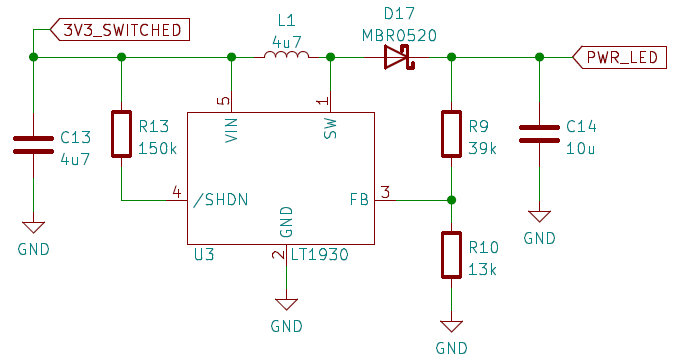
\includegraphics[scale=0.7]{obrazky/LT1930.png}
  \end{center}
  \caption[Zapojení zvyšovače napětí LT1930]{Zapojení zvyšovače napětí LT1930.}
\end{figure}

Pin FB slouží  pro zapojení zpětné vazby napětí na baterii. Jeho referenční napětí musí být nastaveno v~rozmezí 1,240~V až 1,270 V, typická hodnota je však 1,255~V \cite{LT1930_dtsh}. 
Pro výstupní napětí 5 V~byl zvolen rezistor R10 o~hodnotě 13 k$\Omega$ z~rezistorové řady E24 \cite{rezistorova_rada}. Řada E24 byla zvolena kvůli požadované přesnosti
napětí na pinu FB obvodu LT1930. Napětí na rezistoru R10 musí být tedy 1.255 V. Na rezistoru R9 je tedy úbytek napětí 3,745 V. Pomocí trojčlenky byla dopočítána hodnota 
rezistoru R9 dle rovnice:
\begin{equation} 
  R_{9}~=~\frac{R_{10}~\cdot~U_{R9}}{U_{R10}}~=~\frac{13~\cdot~3,745}{1,255}~=~38,79~\:k\Omega. 
  \quad
\label{eq:R9}
\end{equation}

Nejbližší hodnota rezistoru z~rezistorové řady E24 je 39 k$\Omega$ \cite{rezistorova_rada}. Reálná hodnota napětí na rezistoru R10, tj. napětí na pinu FB byla dopočítána
dle rovnice:
\begin{equation} 
  U_{R10}~=~\frac{U_{OUT}}{R_{9}~+~R_{10}}~\cdot~R_{10}~=~\frac{5}{39~+~13}~\cdot~13~=~1,25~V. 
  \quad
\label{eq:UR10}
\end{equation}

Napětí 1,25 V~je v~povoleném rozmezí napětí na pinu FB. 

Přesné výstupní napětí se spočítá podle vzorce:
\begin{equation} 
  U_{OUT}~=~U_{FB}~\cdot~(1~+~\frac{R_{9}}{R_{10}})~=~1,25~\cdot~(1~+~\frac{39}{13})~=~5~V. 
  \quad \quad \quad \quad \cite{LT1930_dtsh}
\label{eq:VOUT_LT1930}
\end{equation}

\section{Zvuková signalizace}
Zvuková signalizace může sloužit například pro potvrzení správnosti hesla, možnosti odejít na další stanoviště, vypršení času pro daný úkol a mnoho dalších. 

Jako zvuková signalizace bylo vybráno piezo s~vlastním oscilátorem typu \\BMT1205XH7.5 \cite{piezo_dtsh}. Maximální odebíraný proud vybraného pieza je 30 mA a rezonanční frekvence 
je 2,3 kHz \cite{piezo_dtsh}. Intenzita zvuku pieza je ve vzdálenosti 10 cm od něj minimálně 83 dB \cite{piezo_dtsh}.

\begin{figure}[!h]
  \begin{center}
    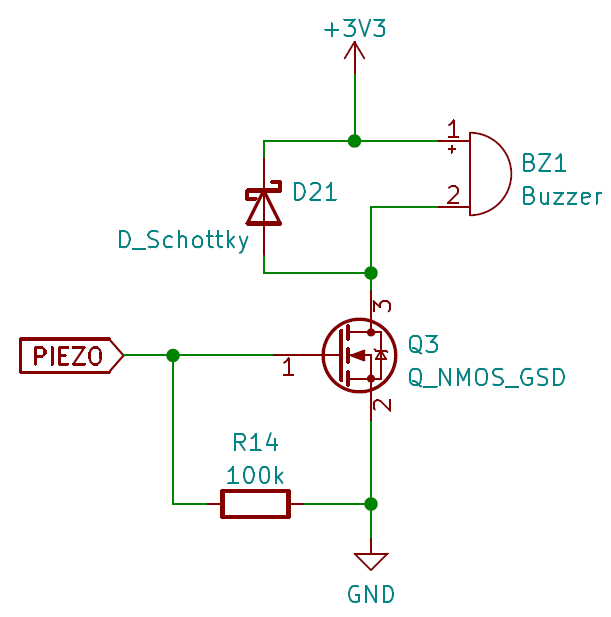
\includegraphics[scale=0.45]{obrazky/piezo.png}
  \end{center}
  \caption[Schéma zapojení pieza]{Schéma zapojení pieza.}
\end{figure}

\section{Konektor}
Jako programovací a zároveň nabíjecí konektor byl zvolen konektor USB-C. Tento konektor je v~dnešní době velmi rozšířený a jeho použití se v~následující době stále rozšiřuje. 

Konektoru USB-C je využíván pouze jako standardní a dostupný konektor, který je mezi běžnou
populací rozšířený a v~následujících letech se bude rozšiřovat stále více. Je využito standardního jmenovitého napětí 5 V~pro nabíjení baterií a nadále pinů D+ a D-, 
které jsou využity pro komunikaci při programování. 

\begin{figure}[!h]
  \begin{center}
    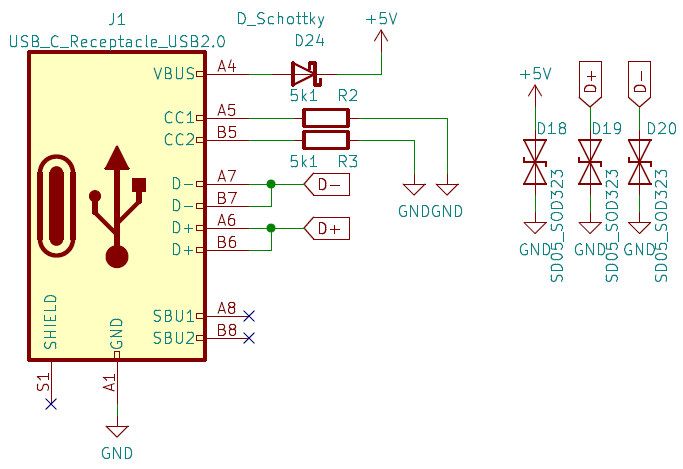
\includegraphics[scale=0.6]{obrazky/USB_C.png}
  \end{center}
  \caption[Zapojení konektoru USB-C]{Zapojení konektoru USB-C.}
\end{figure}

Konektor USB-C je robustní a oboustranný, díky čemuž nebude docházet k~tak častému poškození, jak by mohlo být např. u~konektoru Micro USB. Při používání běžnou veřejností
se jedná o~vítaný bonus. 

Vybraný mikrokontrolér ESP32-C3 umožňuje komunikaci přímo po USB protokolu a není díky tomu zapotřebí žádného převodníku pro komunikaci \cite{ESP_C3_dtsh}.

\begin{figure}[!h]
  \begin{center}
    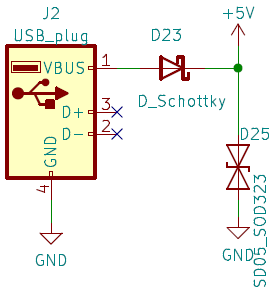
\includegraphics[scale=0.7]{obrazky/USB_A.png}
  \end{center}
  \caption[Zapojení konektoru USB-A]{Zapojení konektoru USB-A.}
\end{figure}

Připojené Shottkyho diody k~napájecímu napětí slouží pro zadržení případného zpětného proudu. Shottkyho diody jsou dimenzovány na proud, který odebírá celé zařízení. Vybrané 
Shottkyho diody  B5819W mají maximální napětí 20 V, jmenovitý proud 1 A~a maximální špičkový proud 9 A~\cite{shotky_dtsh}.

Transily připojené k~napájecímu pinu a ke komunikačním pinům D+ a D- slouží k~ochraně proti přepětí a elektrostatickým výbojům o~velikosti až 30 kV. 

Pro napájení pomocí powerbanky bez potřeby kabelu slouží konektor USB-A. 

Rezistory o~hodnotě 5,1 k$\Omega$ na pinech CC1 a CC2 slouží pro signalizaci, že je k~USB-C připojeno zařízení. Dle standardu USB-C totiž nabíječka bez 
připojení těchto rezistorů nesmí připojit napájecí napětí 5 V~na pin VBUS \cite{USB-C}. 

%ke každé komponentě napsat odběr

\section{Výsledné zapojení}
Pro realizaci Univerzálního modulu byly vybrány následující komponenty: mikrokontrolér ESP32-C3, baterie LiFePO4, nabíjecí obvod CN3056E, konektory USB-C a USB-A,
kapacitní tlačítka s~převodníkem AT42QT1070, inteligentní LED WS2812C s~převodníkem napětí LT1930, piezo, vibrační motor a LoRa modul. LoRa modul komunikuje 
s~mikrokontrolérem pomocí sběrnice UART, převodník pro kapacitní tlačítka pomocí sběrnice $I^2C$ a programování bude probíhat pomocí USB sběrnice. Vše je 
zapojeno dle následujícího blokového schématu. 

\begin{figure}[!h]
  \begin{center}
    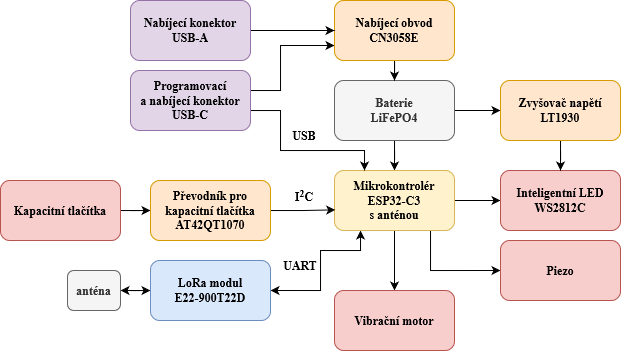
\includegraphics[scale=0.65]{obrazky/vysledne_blokove_schema.png}
  \end{center}
  \caption[Blokové schéma Univerzálního modulu]{Blokové schéma Univerzálního modulu.}
\end{figure}


\chapter{Návrh DPS}
Byl zvolen kruhový tvar desky s průměrem téměř 15 cm a s výběžkem USB-A pro připojení powerbanky. Deska plošného spoje byla navržena v programu KiCad 6.0 a má 2 vrstvy mědi. 
Některé součástky jsou natočeny tak, aby byly co nejvíce na kraji kulaté DPS.

Komunikační dráhy jsou vedeny o tloušťce 0,150 mm a napájecí dráhy jsou vedeny o tloušťce 0,5 mm. Celý návrh byl přizpůsoben výrobním možnostem firmy JLCPCB, kde byla DPS vyrobena.

\section{Kapacitní tlačítka} 
Byl požadavek na 5 tlačítek. Jedno tlačítko je uprostřed a slouží jako hlavní tlačítko. U her bude používáno např. jako registrace průchodu místem apod. Bude tedy nejčastěji
používáno a zároveň může být stisknuto, když hráč běží, takže by mělo být co nejjednodušeji stisknutelné. Proto bylo navrženo větší než zbylá tlačítka. Konkrétně má 
čtvercový tvar se zaoblenými rohy s rozměry 5~$\times$~5~cm. Ostatní tlačítka slouží například jako směrovky, nebo pro vyklikávání nějakého kódu, aby získali nějakou informaci. 
Slouží tedy primárně, když účastník u Univerzálního modulu stojí, nebo sedí, a vyklikává. Díky tomu mohou být tlačítka menší než hlavní tlačítko, konkrétně mají 2~$\times$~2~cm 
a jsou taktéž čtvercová se zaoblenými rohy. Tato tlačítka jsou proto umístěna po stranách hlavního tlačítka a jsou popsána BTN\_ENTER, BTN\_UP, BTN\_DOWN, BTN\_RIGHT a BTN\_LEFT.

V oblastech kapacitních tlačítek nejsou umístěny žádné další součástky a v jejich okolí je rozmístěna země kvůli odstínění. 

Pod spodním tlačítkem je ze spodní strany umístěno pouzdro na baterii. Kdyby bylo pouzdro až pod tlačítkem, musel by se ještě hodně zvětšit průměr DPS. Pokud by se při testování 
prototypu ukázalo, že kvůli umístění pouzdra baterie dochází k rušení tlačítka, tak dojde při výsledné verzi DPS k posunutí pouzdra baterie. 

\section{LED}
Po obvodu DPS je poté rovnoměrně rozmístěno do kruhu všech 12 programovatelných LED. Takto rozmístěné LED mohou zobrazovat např. podíl uběhnutého času. 12 LED bylo zvoleno z důvodu 
možnosti rozdělení na 2, 3 nebo i 4 segmenty. Na 12ti LED v kruhu lze také zobrazovat čas.

\section{Ostatní součáskty}
Ze zadní strany DPS je umístěna veškerá řídicí elektronika. Ve spodní straně je umístěno pouzdro s baterií LiFePO4 a v jeho blízkosti je umístěn nabíjecí obvod. V levém 
spodním rohu je poté umístěn konektor USB-C, který slouží pro nabíjení baterie a zároveň pro programování. Nad pouzdrem pro baterii je umístěn zvyšovač napětí pro programovatelné 
LED a nedaleko jsou LED diody indikující přítomnost napájecího napětí 3,3 V a 5 V. Ze zadní strany je v levé horní části umístěn mikrokontrolér ESP32-C3 a v pravé horní části 
LoRa modul. Nad tlačítky je umístěn převodník pro kapacitní tlačítka AT42QT1070-S.

Otvory pro připojení vypínače jsou umístěny u konektoru USB-C a otvory pro připojení vibračního motoru jsou umístěny mezi LoRa modulem a vrchním tlačítkem BTN2\_UP1. 

Z přední strany DPS je také umístěn bzučák. 

\section{Průběh návrhu}
Při návrhu DPS byla dodržována pravidla a konvence dobrého návrhu DPS.

V oblasti antény od ESP32-C3 mikrokontroléru nejsou taženy žádné dráhy, ani pod ní není rozlitá žádná měď. Je to z důvodu zaručení většího dosahu signálu a pro snížení rušení. 

Filtrační kondenzátory jsou vždy umístěny co nejblíže pouzdrům daných čipů. Shottkyho diody jsou umístěny v blízkosti USB konektorů. Rozmístění součástek kolem zvyšovače napětí 
je provedeno dle doporučení z dokumentace. 

Komunikační piny D+ a D- pro programování jsou taženy jako diferenciální pár.

\chapter{Osazení, oživení a testování DPS}
Výrobní podklady byly vygenerovány pomocí programu Kikit. Deska byla vyrobena u firmy JLCPCB, protože je bezkonkurenčně nejlevnější a její dodání je rychlé a bezproblémové. 
Jejich výrobky také dosahují vysoké kvality. 

\begin{figure}[!h]
  \begin{center}
    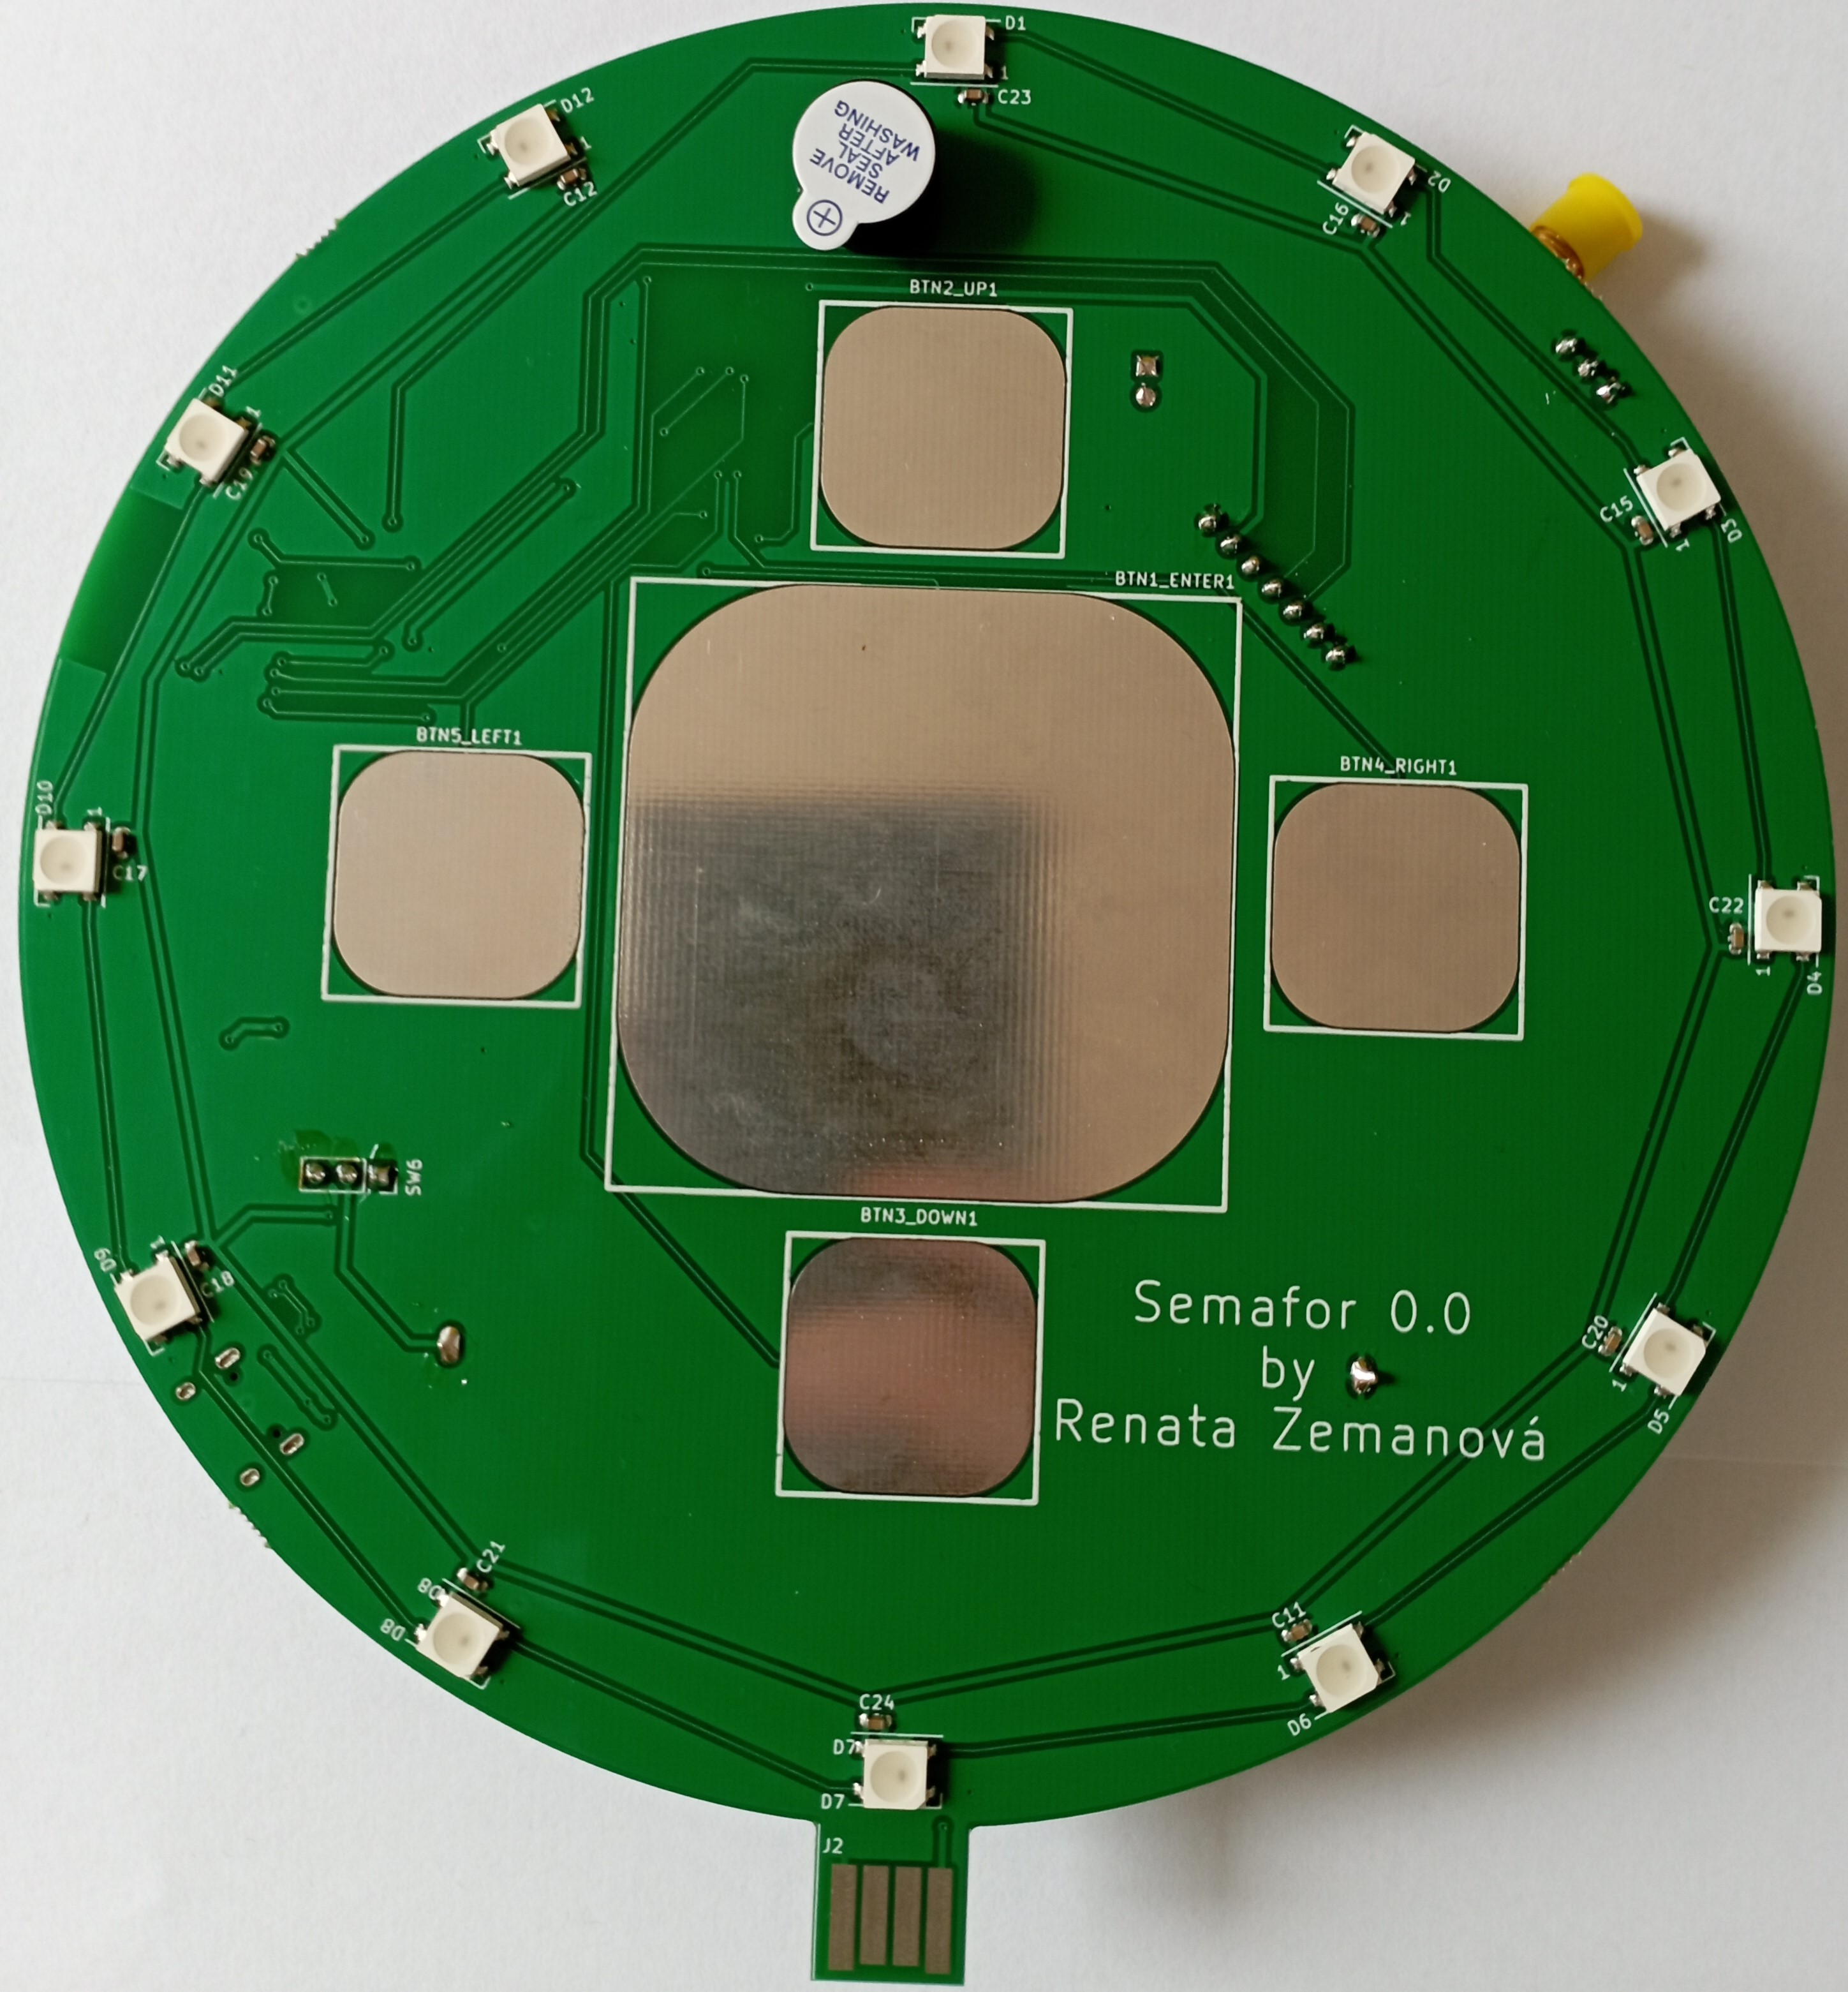
\includegraphics[scale=0.13]{obrazky/DPS_prototyp_top.jpg}
  \end{center}
  \caption[Výsledná DPS prototypu - přední strana]{Výsledná DPS prototypu - přední strana.}
\end{figure}

DPS byla taktéž strojově osazena u firmy JLCPCB. Z důvodu nedostupnosti některých součástek byly některé komponenty zakoupeny v jiných obchodních řetězcích a doosazeny ručně. 
Jednalo se o držák na baterie, piezo, kondenzátor C3 v pouzdře 0805 o hodnotě 100 $\mu$F, čip pro kapacitní tlačítka AT42QT1070, vypínač a LoRa modul. 

Nebyl sehnán přesný typ držáku, pro který byl Univerzální modul navržen, proto byly nožičky držáku roztaženy, aby byla jejich rozteč zvětšena a mohlo dojít k zapájení. U pieza také chybělo 
označení polarity. Do finální verze bylo tedy přidáno do popisové vrstvy plus u správného vývodu. Vypínač byl kvůli testovacím účelům realizován pinheady a na ně byla nasazena 
propojka. Na místo LoRa modulu byly připájeny dutinky a LoRa modul byl pouze zasunut do dutinek. Hlavním důvodem byla cena tohoto modulu. LoRa modul bude z prototypu přesunut 
na finální výrobek a nedojde tak k plýtvání součástek ani peněz.

\begin{figure}[!h]
  \begin{center}
    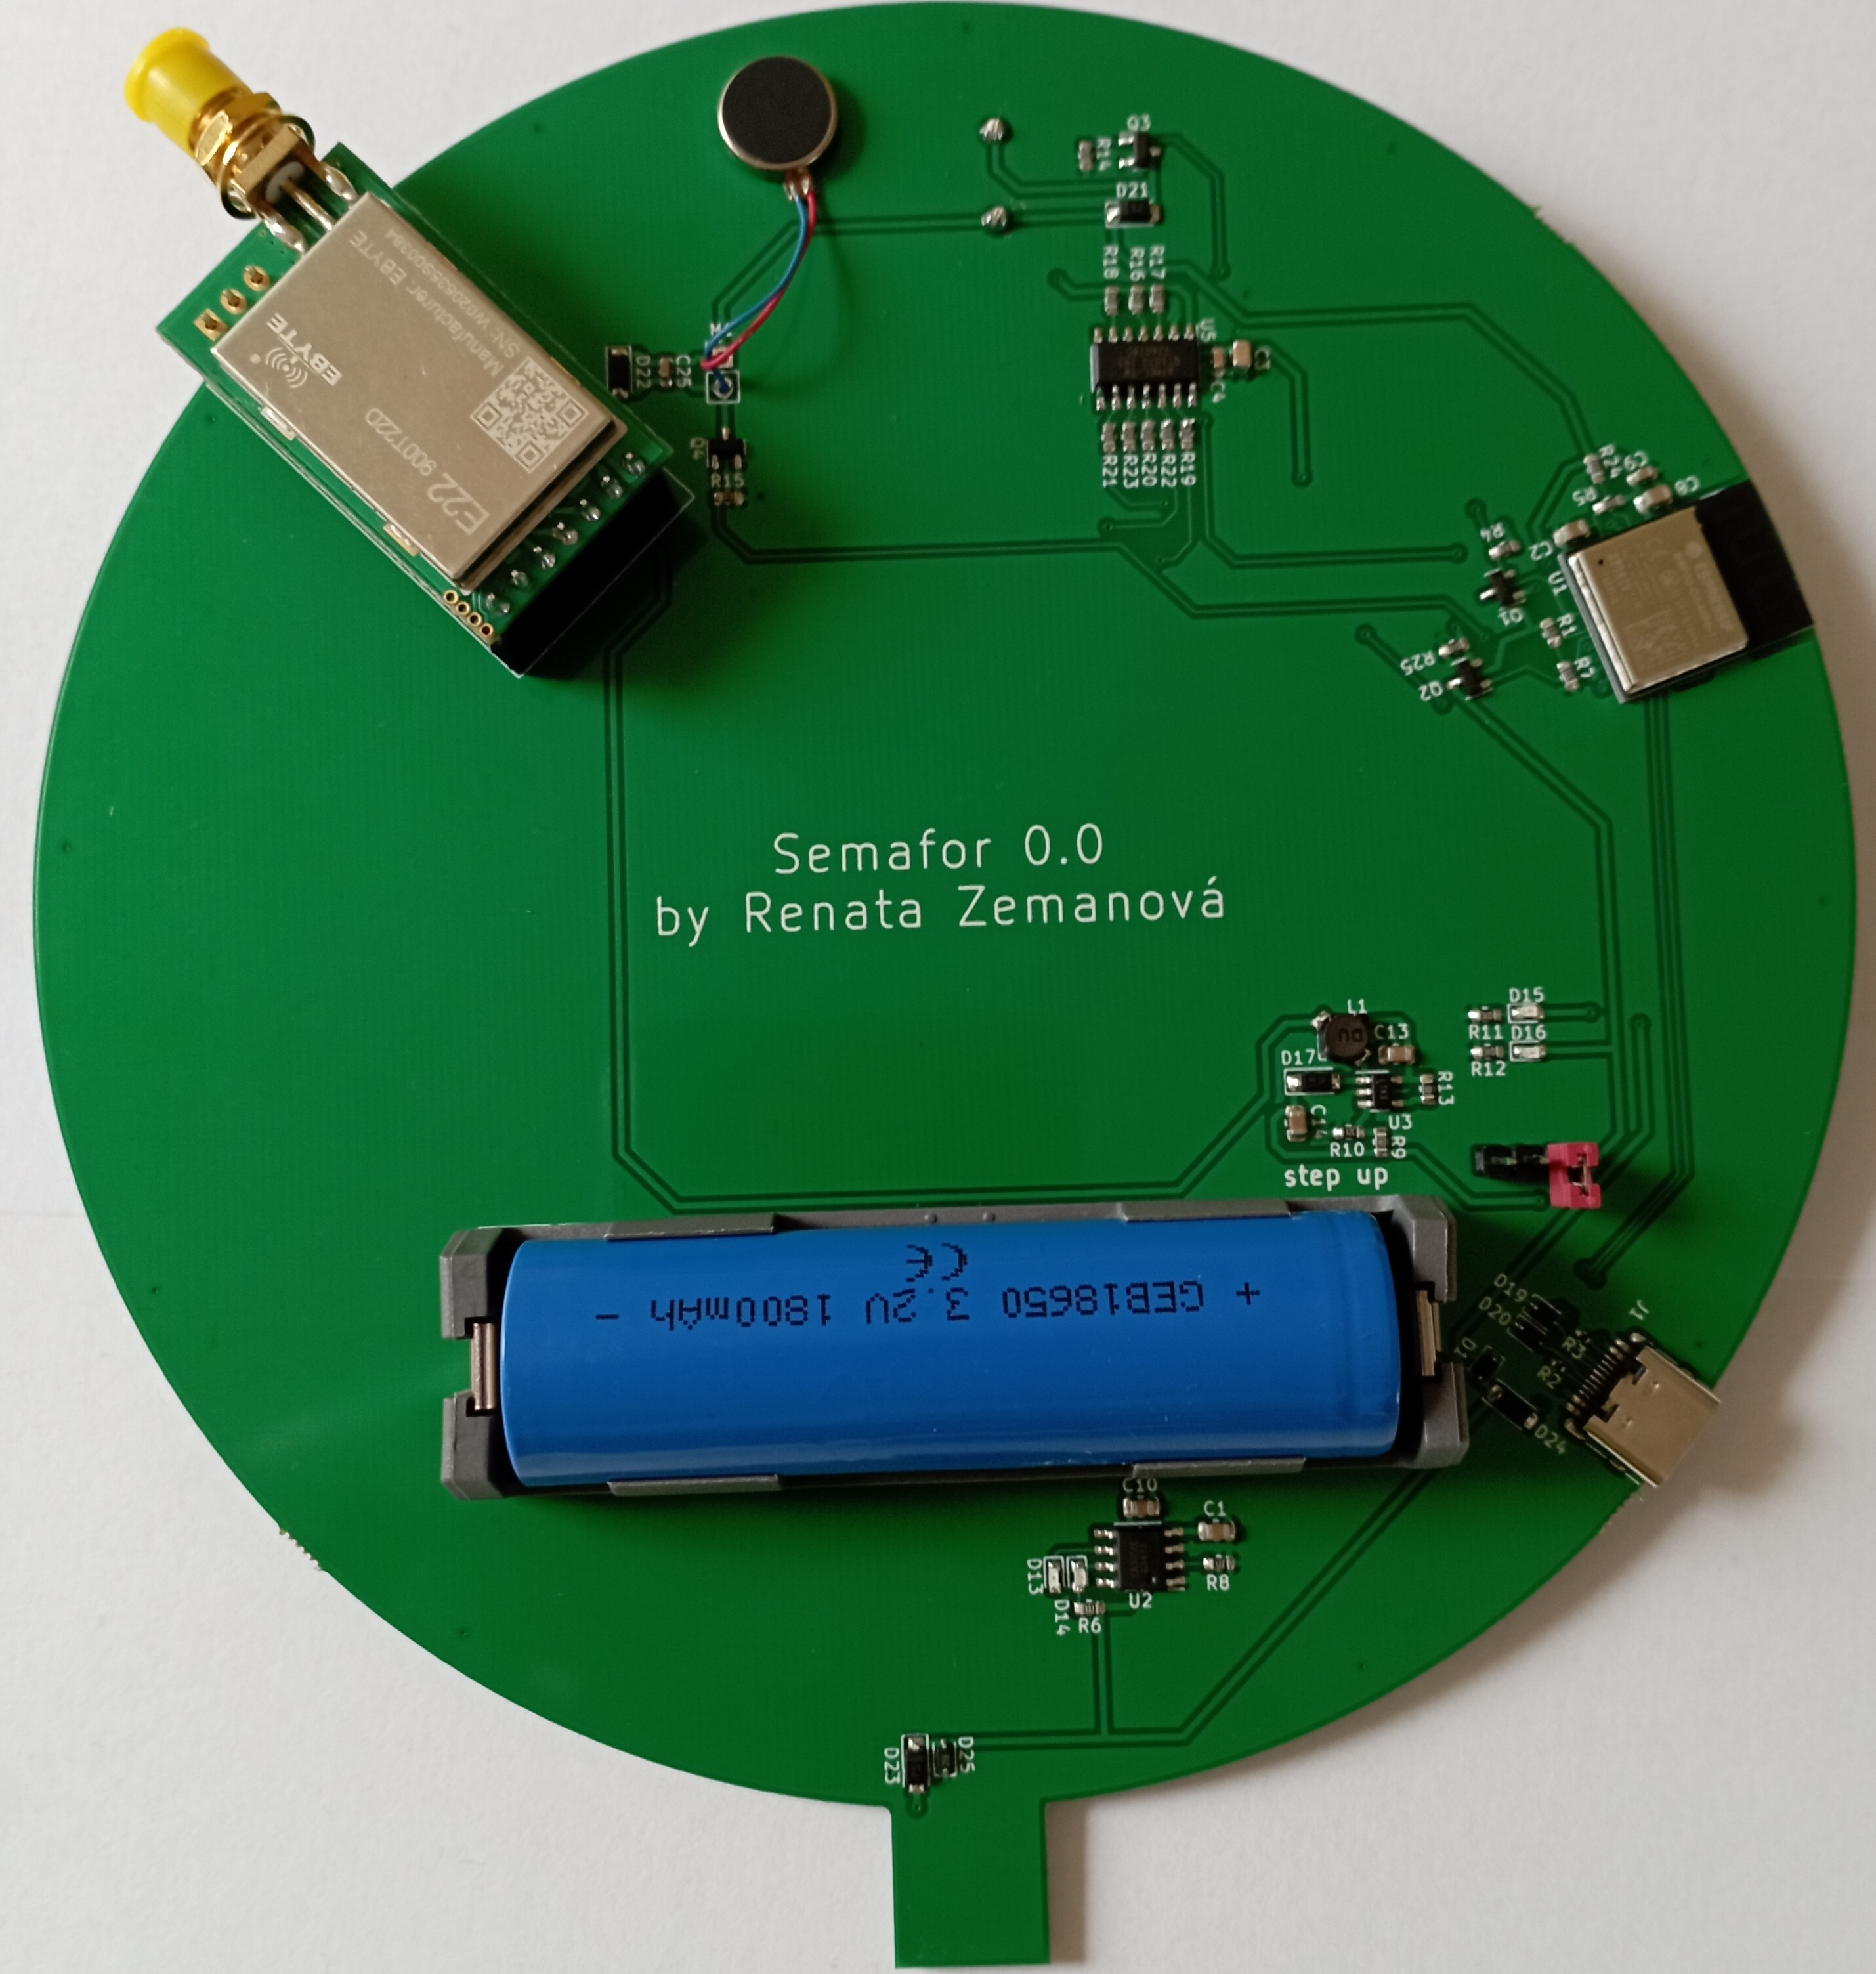
\includegraphics[scale=0.13]{obrazky/DPS_prototyp_bottom.jpg}
  \end{center}
  \caption[Výsledná DPS prototypu - zadní strana]{Výsledná DPS prototypu - zadní strana.}
\end{figure}

\section{Oživení}
Po připájení všech součástek byla do pouzdra vložena baterie LiFePO4 a DPS byla pomocí propojky zapnuta. Po zapnutí DPS se rozsvítila LED indikující přítomnost napětí 3,3 V. 
Po připojení konektoru USB-C s napájecím napětím se rozsvítila i LED indikující napětí 5 V. Také se rozsvítila červená LED indikující nabíjení baterie. Baterie byla pod dohledem 
nabíjena v DPS. Nedošlo k zahřátí DPS ani baterie a po čase se u nabíjecího obvodu rozsvítila místo červené LED zelená LED. Tato LED indikuje plně nabitou baterii. Na plně nabité 
baterii bylo naměřeno napětí 3,4 V. Nabíjecí obvod byl tedy otestován a bylo zjištěno, že funguje správně. 

Při měření napětí bylo zjištěno, že napájecí napětí pro programovatelné LED dosahuje pouze 1,7 V. Dalším měřením bylo zjištěno, že ani na vstupu zvyšovače napětí není 3,3 V, ale 
pouze 1,7 V. Díky tomu bylo zjištěno, že při logické 1 na pinu IO5 je 3,3 V, ale na spínaném výstupu je pouze 1,7 V. Bylo zjištěno, že byl použit tranzistor typu NMOS, který nelze 
v takovém zapojení plně otevřít. Tranzistor tedy zůstává v lineárním režimu, a proto je na výstupu pouze 1,7 V. Chyba byla vyřešena výměnou tranzistoru. Místo NMOS byl použit PMOS 
a do finální verze byla chyba opravena. Byla vyměněna schématická značka tranzistoru za PMOS a zároveň byl vyměněn kód součástky, aby byla správná součástka osazena již u firmy JLCPCB. 

Po opravě již mělo napájecí napětí pro inteligentní LED hodnotu 5 V. Díky tomu bylo zjištěno, že zvyšovač napětí funguje správně. 

\section{Testování}
DPS byla naprogramována a komunikace mezi počítačem a mikrokontrolérem proběhla bezproblémově. Byl napsán testovací SW pro programovatelné LED 
a další periferie. Díky tomu mohly být otestovány programovatelné LED. Všechny inteligentní LED bylo možné rozsvítit různými barvami, takže jsou plně funkční. Byla otestování funkčnost 
zapojení pieza a vibračního motoru. Obě zapojení byla funkční. 

Dále bylo testováno zapojení kapacitních tlačítek a jejich čtení. Pro komunikaci s čipem AT42QT1070 byla použita knihovna AtTouch, která je primárně určena pro Arduino \cite{AtTouch}. 
Knihovny pro Arduino bývají převážně s mikrokontroléry ESP32 kompatibilní. Nejdříve bylo zjištěno, že knihovna předpokládá připojení I2C na konkrétních pinech, tj. SCL na GPIO9 a SDA 
na GPIO8 \cite{AtTouch}. Mnou navržený Univerzální modul má piny připojené naopak, tj. SCL na GPIO8 a SDA na GPIO9. Došlo tedy k upravení knihovny, aby jako vstupní parametry byly přebírány i GPIO 
piny I2C. Testovací software, který používal upravenou knihovnu AtTouch ale nebyl funkční. Nedocházelo k detekci stisku tlačítka a ani pin /CHANGE neměnil svůj stav. Ani po zapnutí 
softwarového pullup rezistoru nezačal pin /CHANGE generovat správné pulzy. Proto byla DPS 
připojena k osciloskopu. Nejdříve byla sledována komunikace po I2C pomocí pinů SCL a SDA. Díky tomu bylo zjištěno, že počáteční ustavovací komunikace probíhá v pořádku a mikrokontrolér 
se s čipem AT42QT1070 domluví. Díky tomu bylo zjištěno, že čip AT42QT1070 funguje správně, ale data jsou knihovnou AtTouch chybně zpracovávána. Tato knihovna také neumožňovala detekci 
stisků více tlačítek současně, i když tuto funkci použitý čip AT42QT1070 umí. Z tohoto důvodu bylo rozhodnuto, že bude mnou vytvořena nová knihovna, která bude tuto funkci podporovat 
a budou v ní odstraněny všechny chyby, které jsou v knihovně AtTouch. 

Při tvorbě knihovny bylo zapotřebí otestovat funkci jednotlivých registrů. Registr Detection Status generuje při doteku jakéhokoli tlačítka jedničku na bitu nula. Zároveň, pokud je tento 
registr čten, tak pin /CHANGE negeneruje pulzy a zůstává v klidové pozici, tj. logické jedničce. Bylo tedy rozhodnuto, že pokud se bude daná informace používat, tak to bude právě z registru 
Detection Status a díky tomu se uvolní pin na mikrokontroléru, který bude moci být použit pro připojení dalších periferií. Registr Key Status indikuje pouze stisk jednoho tlačítka. Pokud 
je jich stisknuto více, tak se celý vynuluje. Toto chování může být způsobeno velikostí kapacitních tlačítek, jejich návrhem, nebo může být chyba v čipu AT42QT1070. Registry Key Signal 
uchovávají aktuální měřenou informaci o měřené kapacitě ve 2 bytech pro každé tlačítko. Tyto hodnoty se mění v závislosti na prostředí, ve kterém se Univerzální modul nachází, a také v závislosti 
na stisknu. Při stisku jsou hodnoty změněny skokově a hodnota měřené kapacity se výrazně změní. 
Registry Reference Data uchovávají data po kalibraci. Při testování se stávalo, že se kalibrace spouštěla sama ve chvílích, kdy bylo některé z tlačítek stisknuto. Zejména dělalo problémy hlavní
velké tlačítko. Proto byla v knihovně využívána data pouze z registrů Key Signal a změna byla detekována pouze pomocí tohoto registru. Díky tomu, že změna prostředí nedělá tak velké a prudké 
změny. Tlačítka byla nadále rozdělena do jednotlivých skupin, aby mohl být detekován i multistisk. To bylo nastaveno v registrech AVE/AKS. Bity 0 a 1 byly nastaveny do nuly, což znamená, že 
tlačítka nejsou v žádné skupině, takže je každé samostatně. Pro používaná tlačítka 0 až 4 byly nastaveny registry na hodnotu 32, což znamená, že měřená hodnota je průměrem z 8mi naměřených
hodnot. Registry pro tlačítka 5 a 6 jsou vynulovány, a tím jsou tyto vstupy deaktivovány. 

Pro práci s kapacitními tlačítky jsou tedy primárně využívány registry Key Signal a informace o stisku jsou z nich dopočítávány. 

Byla otestována komunikace s E22-900T22D LoRa modulem. Vyčítání informací z LoRa modulu probíhalo v pořádku, ale kvůli nepřipojení pinů M0, M1 a AUX k mikrokontroléru nemohl být Univerzální modul 
nastaven tak, aby komunikoval s dalšími Univerzálními moduly. Tyto chyby byly opraveny do finální verze a další testování tohoto Univerzálního modulu probíhalo až na hardwaru finální verze DPS. 
%testování LoRa modulu

\chapter{Finální verze DPS}
Finální verze DPS byla zmenšena na průměr 10 cm, protože DPS od firmy JLCPCB jsou mnohem levnější, když mají maximální rozměry 10$\times$10 cm. Také jejich skladovací nároky jsou mnohem  menší. 
Kvůli tomuto zmenšení ale nebylo dost místa 
kolem kapacitních tlačítek, aby nedocházelo k jejich rušení z okolních obvodů. Zároveň by musela být tlačítka moc blízko u sebe, takže by mohlo docházet k jejich přeslechům. Routování takové 
DPS, aby dráhy nevedly v blízkosti kapacitních tlačítek ani pod nimi bylo takřka nemožné. Proto bylo přistoupeno k řešení 2 spojených DPS. Díky tomu mohly být obě DPS osazeny pouze z jedné strany,
což ušetří další nemalé peníze. I při výrobě 2 kusů DPS o průměru 10 cm místo jedné velké byla cena výhodnější. Na spodní DPS je tedy veškerá řídicí elektronika a na vrchní DPS jsou pouze tlačítka 
a programovatelné LED. Kolem kapacitních tlačítek byla také vytvořena tzv. ochranná zóna, která slouží pro lepší odstínění tlačítek od ostatních signálů \cite{conv_cap_but_AT42QT1070_dtsh}. Tato zóna 
byla připojena k převodníku AT42QT1070 dle datasheetu na pozici prvního tlačítka - pin KEY0 \cite{conv_cap_but_AT42QT1070_dtsh}. 

Po konzultaci bylo domluveno, že při napájení z baterie a možnosti napájení přes konektor USB-C není konektor USB-A zapotřebí. Rozměry DPS by se tím také opět zvětšily a výrobní náklady by tím 
stouply. 

Do finální verze byl také přidán fototranzistor, který bude následně využíván pro automatickou regulaci jasu programovatelných LED typu WS2812C. Fototranzistor byl připojen na GPIO01 mikrokontroléru ESP32-C3. Na tomto 
pinu je k dispozici AD převodník \cite{ESP_C3_dtsh}. Byl vybrán fototranzistor s označením SMD3528C-50, který je citlivý na viditelné světlo \cite{Phototransistor}.
Tento fototranzistor byl umístěn také na vrchní DPS. 
%schéma zapojení fototranzistoru

Dále byl také 
přidán konektor pro připojení dalších programovatelných LED typu WS2812C, které mohou být na pásku připevněném po obvodu Univerzálního modulu. Tyto LED mohou zajišťovat, aby Univerzální modul mohl svítit 
nejen dopředu, ale i do stran. Tato funkcionalita opět rozšíří možnosti využití tohoto Univerzálního modulu. Na datový pin těchto programovatelných LED byl připojen do série ochranný rezistor, který 
zabraňuje zničení pinu mikrokontroléru EPS32-C3, kdyby byly omylem zkratován s napájecím napětí. 

Bylo zapotřebí připojit k mikrokontroléru i piny M0, M1 a AUX od LoRa modulu E22-900T22D. Na mikrokontroléru ale nebylo již dostatek volných GPIO pinů, a tak byl použit expander GPIO pinů. Vybraný expander
PCA9536D umožňuje připojení 4 GPIO a zároveň komunikuje s mikrokontrolérem přes sběrnici $I^2C$ \cite{expander}. Pin AUX byl tedy připojen k mikrokontroléru přímo přes GPIO05 a piny M0 a M1 byly připojeny k GPIO0 
a GPIO1 expanderu. Protože byly ještě volné GPIO piny na expanderu, bylo realizováno ještě samostatné vypínání napájení programovatelných LED, protože i když tyto LED nesvítí, tak mají stále spotřebu 
0,3 mA na jednu LED \cite{WS2812C_dtsh}. Při bateriově napájené aplikaci je to stále nemalý proud, a proto byl realizován právě tento samostatný vypínač napájení. 
%schéma zapojení expanderu

Ve finální verzi DPS byl použit posuvný vypínač se zahnutými vývody. Díky tomu mohl být vypínač umístěn na okraj DPS a nemusel být ručně pájen na drátkách. LED indikující přítomnost napájecího napětí 
3,3 V a LED indikující nabíjení nebo plné nabití baterie byly dány na okraj spodní DPS tak, aby bylo možné je vidět, ale zároveň aby při používání Univerzálního modulu při hře nemohly zmást. LED indikující přítomnost 
napájecího napětí 5 V byla odstraněna pro její nadbytečnost. 

Byly přidány také zkratovací prokovy na EN pinu mikrokontroléru s GND. Při zkratování je restartován mikrokontrolér. Tyto prokovy slouží pro snazší oživování a testování softwaru. Při provozu nebude propojka 
zkratována a bude zabráněno jejímu náhodnému zkratování. 

%změny  na GPIO pinech, kam bylo co přepojeno, proč to mohlo být přepojeno

%odůvodnit pozici baterie

\begin{figure}[!h]
  \begin{center}
    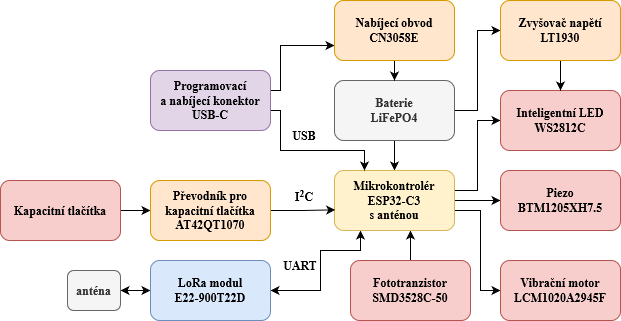
\includegraphics[scale=0.65]{obrazky/blokove_schema_finalni_verze.png}
  \end{center}
  \caption[Výsledné blokové schéma Univerzálního modulu]{Výsledné blokové schéma Univerzálního modulu.}
\end{figure}

Při návrhu byly také brány v potaz tekoucí proudy danými drahami. Tloušťky drah tomu byly přizpůsobeny a případné prokovy také. Například dráhy od baterie, jak k nabíjecímu obvodu, tak k USB mají tloušťku
2 mm, signálové dráhy mají tloušťku 0,125 mm a ostatní napájení dráhy mají tloušťku 1 mm. Prokovy mají vždy vrtanou díru stejně velkou, jako je tloušťka dráhy a okolní měď má průměr alespoň o 0,2 mm větší 
než vrtaná díra. U dvounožičkových součástek byl také řešen thombstone efekt. Proto u takových součástek byly dráhy vyvedeny stejně tlusté, případně alespoň co nejpodobnější. 
%obrázek řešení thombsone efektu - původní a řešení 

Rozložení součástek zvyšovače napětí bylo realizováno dle doporučení z datasheetu. Prokovy k signálu GND byly umístěny co nejblíže k vstupnímu i výstupnímu kondenzátoru. Propojovací konektory byly 
umístěny po obvodu a byly na ně připojeny všechny potřebné signály. Napájecí napětí a GND signál byly přivedeny přes jeden konektor, aby se tak zlepšilo EMC. 

%Blokové schéma finální verze

\section{Výroba a oživení}

DPS byla následně opět vyrobena a osazena u firmy JLCPCB. Opět nebyly k dispoziciu firmy JLCPCB všechny potřebné součástky, takže některé byly osazeny ručně. Šlo o XXX.
%propojení DPS realizováno prodlouženými pinheady, aby se mezi DPS vešla baterie. 
%napsat co jsem ručně osazovala
%napsat i oživení 

%fotka vyrobené a hotové DPS finální verze

\chapter{Firmware}
V následující kapitole je popsán firmware Univerzálního modulu. Jsou zde popsány funkce, které byly vytvořeny pro následnou tvorbu softwaru Univerzálního modulu a pro usnadnění práce s ním. Univerzální 
modul je programován v jazyce C++ a je využit Arduino framework, který mikrokontroléry ESP32 podporují.  

\section{Hlavní knihovna}
Hlavní knihovna sdružuje veškeré funkce, které jsou Univerzálnímu modulu k dispozici. Tato knihovna obsahuje funkce pro práci s kapacitními tlačítky, programovatelnými LED, WiFi, piezem, vibračním 
motorem i fototranzistorem. 

Pro práci s programovatelnými LED byla využita knihovna Adafruit\_NeoPixel.h. V hlavní knihovně byly vytvořeny funkce, které umožňují rozsvítit konkrétní barvou jednotlivé LED nebo všechny současně. Také 
je lze jednotlivě nebo všechny zhasnout. Byly vytvořeny také funkce pro blikání. 

Pro práci s tlačítky byly implementovány funkce, které zjišťují, zda je některé z tlačítek stisknuto. Každé tlačítko má svoji funkci. V některých případech není zapotřebí vědět, které z tlačítek je stisknuto, 
ale zda je vůbec některé z nich stisknuto. Pro tyto účely vznikla funkce, která to umí zjistit. 

Dále byly vytvořeny funkce pro zapnutí a vypnutí pieza a zároveň pro zapnutí a vypnutí vibračního motoru. 

%LoRa - asi nebude

%WiFi

Pro hlídání stavu nabití baterií byly vytořeny funkce, které měří napětí na baterii a zjišťují, zda je baterie dostatečně nabitá, či nikoli. 

Dále knihovna obsahuje funkci pro vypnutí napájení periferiím, které jsou náročnější na spotřebu. Tato funkce může být využita právě při indikaci nízkého bateriového napětí.

\section{Práce s kapacitními tlačítky}
Pro převodník AT42QT1070, který převádí signál z kapacitních tlačítek na komunikaci po sběrnici $I^2C$, byla připravena knihovna AT42QT1070.h. Tato knihovna obsahuje 3 třídy, které dopomáhají 
práci s tlačítky a usnadňují ji. 

Třída s názvem AT42QT1070Touch obsahuje funkci begin, která slouží pro nastavení čipu AT42QT1070, rozděluje tlačítka do jednotlivých skupin a dělá počáteční kalibraci. Z tohoto důvodu nesmí být při 
zapnutí Univerzálního modulu stisknuto žádné tlačítko. Pokud by tomu tak bylo, tak by se tlačítka chybně zkalibrovala a docházelo by tak k falešným stiskům. Funkce tick musí být volána pravidelně, aby docházelo 
k neustálé obnově dat a kalibraci tlačítek. Díky tomu nejsou vyvolány falešný stisky při změně prostředí, která může způsobovat pozvolnou změnu kapacity. Funkce get\_raw\_data\_btn bere jako parametr 
index tlačítka a vrátí hodnotu kapacity tlačítka přímo z registru čipu AT42QT1070. Funkce is\_touched\_btn přebírá jako parametr index tlačítka a vrací informaci o tom, zda je tlačítko stisknuto 
či nikoli.  

Třída s názvem TouchButton reprezentuje tlačítko. V této třídě je definována funkce tick, která přebírá aktuální vzorek z tlačítka. Tento vzorek je porovnáván s průměrně naměřenou hodnotou. Pokud 
je aktuálně naměřená hodnota blízká průměrné hodnotě, tak je tento vzorek započítán do průměru. Pokud je aktuálně naměřená hodnota dostatečně rozdílná oproti předchozím průměru, tak je detekován stisk. 
Stisk je signalizován až ve chvíli, když je neměřen 3$\times$ za sebou. Díky tomu jsou vyloučeny falšené stisky, které mohou být vyvolány například okolním rušením.  

Třída s názvem MovingAverage slouží pro počítání klouzavého průměru z naměřených hodnot z tlačítek. Funkce push\_sample převezme naměřený vzorek a nahradí jím nejstarší vzorek, který je pro počítání 
průměru využit. Funkce setup přebírá 2 parametry. První parametr size určuje, z kolika posledních naměřených vzorků bude průměr počítán, a druhý parametr initial\_value udává první hodnoty, které 
jsou po spuštění využity pro počítání průměru. Při použití jsou poté předávány hodnoty z počáteční kalibrace. 

\section{Webový server}

%pak upravit, podle skutečnosti
Pro práci s WiFi byla vybrána knihovna WiFi.h, která je určena pro Arduino i mikrokontroléry typu ESP32 \cite{WiFi_lib}. Testovací kód obsahoval vytvoření WiFi sítě a následně vytvoření webové 
stránky. Telefon byl připojen k vytvořené WiFi síti a poté byl přesměrován na vytvořenou webovou stránku. Dále probíhalo testování získávání dat z nastavení na webové stránce. 
%dopsat všechno, co jsem do teď udělala


%celkovy popis FW

\section{Celková funkce}
Univerzální modul po zapnutí nastaví všechno GPIO na vstupní nebo výstupní dne potřeby, případně zapne softwarové pullup rezistory. Poté je načtena konfigurace z permamentní paměti. V té je uložena poslední hra 
i s její konfigurací. Pokud je Univerzální modul spouštěn poprvé, tak je načtena výchozí přednastavená hra s nějakou konfigurací. Zároveň je tato konfigurace uložena do permanentní paměti. Po dalším startu 
Univerzálního modulu pak bude z permanentní paměti načítána poslední konfigurace. 

Poté je nastaven odpočet doby, po kterou může být přepnut Univerzální modul do konfiguračního módu. Tento čas je nastaven proto, aby se při hře nemohlo omylem stát, že by byl Univerzální modul přepnut do 
konfiguračního módu, protože do tohoto módu se přechází kombinací stisknutých tlačítek. 

Univerzální modul pak přechází do herního módu. V herním módu je neustále dokola spouštěna hra, která byla nastavena v konfiguraci. Zároveň, pokud ještě nevypršel čas, do kdy je možné přejít do režimu konfigurace, tak 
je kontrolováno, zda není stisknuta kombinace tlačítek, kterou je zapnut konfigurační mód. V každém cyklu je také čten stav tlačítek. Tato funkce je důležitá pro správné vyhodnocování stisku kapacitních tlačítek. 

Pokud jsou na Univerzálním modulu stisknuta tlačítka "UP" a "DOWN" současně, tak je Univerzální modul přepnut do konfiguračního módu. Tento mód je signalizován blikáním všech LED modrou barvou. V tomto módu je zapnuta WiFi a server. Na 
tuto WiFi se lze připojit telefonem nebo notebookem. Po připojení k WiFi a napsání IP adresy Univerzálního modulu je načtena webová stránka s konfiguračním menu Univerzálního modulu. Po nastavení parametrů dané hry a stisku 
tlačítka pro spuštění dnaé hry je konfigurace sdílena pomocí WiFi. Konfigurace je tak k dispozici ke stažení pro další Univerzální moduly, které jsou v blízkosti konfigurovaného Univerzálního modulu a neuběhl u nich daný čas o jejich 
startu. Následně je server i WiFi vypnuta a Univerzální modul přechází zpět do herního módu. Je spuštěna hra, která byla nakonfigurována. Konfigurace této hry je uložena do permanentní paměti.

%předělat, aby to nebylo dolů, ale doprava
\begin{figure}[!h]
  \begin{center}
    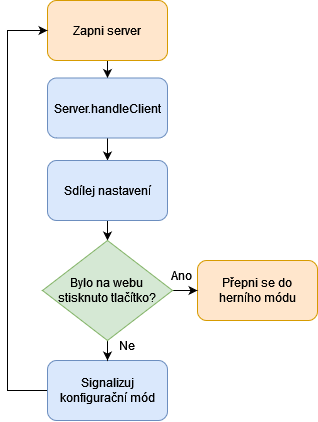
\includegraphics[scale=0.75]{obrazky/blokove_schema_modu_CONFIGURATION.png}
  \end{center}
  \caption[Blokové schéma konfiguračního módu]{Blokové schéma konfiguračního módu.}
\end{figure}

Pokud je dostupná WiFi jiného Univerzálního modulu, tak je Univerzální modul připojen na tuto WiFi a snaží se z ní stáhnout novou konfiguraci. Pokud se podaří konfiguraci stáhnout, tak je zapnuta hra s konfigurací,
která byla stažena z WiFi jiného Univerzálního modulu. Konfigurace této hry je uložena do permanentní paměti. Stažení nové konfigurace je signalizováno půlvteřinovým probliknutím všech LED modrou barvou. 

Přepnutí do konfiguračního módu nebo stažení konfigurace z jiného Univerzálního modulu je možné pouze 5 minut po zapnutí. 

\begin{figure}[!h]
  \begin{center}
    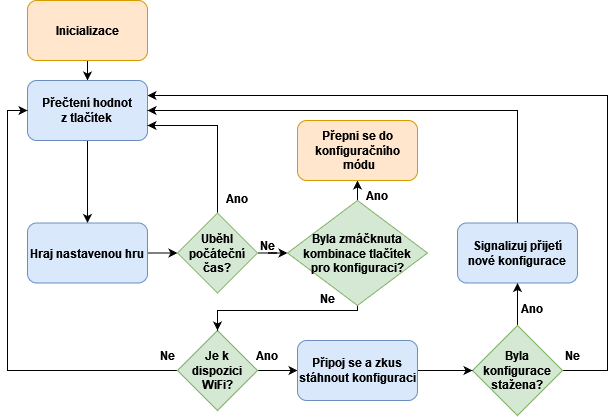
\includegraphics[scale=0.65]{obrazky/blokove_schema_modu_PLAY.png}
  \end{center}
  \caption[Blokové schéma herního módu]{Blokové schéma herního módu.}
\end{figure}

\chapter{Hry a jejich metodika}

\section{Odpočítávadlo}
%o hře - k čemu je možno využít
\underline{Funkce Univerzálního modulu ve hře:}

V konfiguraci je nastavena délka časového limitu. Poté je vysvícena dvanáctina času, který zbývá do konce časového limitu. Stisknutím prostředního tlačítka je odpočet zastaven. 
Zastavení času je signalizováno blikáním daného počtu LED červenou barvou. Opětovným stiskem prostředního tlačítka odpočet pokračuje. 

\section{Vábnička}
%o hře
\underline{Funkce Univerzálního modulu ve hře:}

Hru Vábnička lze hrát ve třech režimech. Nastavení režimu probíhá v konfiguračním menu. 

Režimy hry Vábnička: 
\begin{itemize} 
  \item Boční tlačítka mají charakter barev jednotlivých týmů. Po zmáčknutí daného tlačítka se Univerzální modul rozsvítí danou barvou. 
  \item Středové tlačítko slouží pro přepnutí barvy na náhodnou jinou barvu, než kterou Univerzální modul svítil do teď.  
  \item Středové tlačítko slouží pro přepnutí barvy na následující barvu, která je aktuálně v pořadí. 
\end{itemize}	
V konfiguraci lze také zapnout probíhání kontroly, aby jednotlivé Univerzální moduly nikdy nesvítily všechny stejnou barvou. Alespoň jeden Univerzální modul musí svítit jinou 
barvou než ostatní. K tomu slouží komunikace mezi jednotlivými Univerzálními moduly.

%předchozí kapitola tam nebude, je nahrazena kapitolou Módy a využití

\chapter{Módy a využití}
V této kapitole jsou popsány jednotlivé módy, které byly pro Univerzální modul vyvinuty, jako příklad využití tohoto zařízení. Všechny parametry, které dané módy přebírají, jsou zadávány 
v rámci nastavení na konfigurační webové stránce.

\section{Klasický semafor}
Tento herní mód přebírá jako parametry minimální a maximální čas změny barvy svícení. 

Na začátku hry se s pravděpodobností 0,5 rozsvítí všechny LED zelenou nebo červenou barvou. Následně je nastaven odpočet času, který je náhodný v rozmezí minimálního a maximálního času změny. 
Po uplynutí tohoto času svítí na polovině LED žlutá barva. Na druhé polovině zůstává původní barva. Tento stav trvá 2 sekund. Následně se všechny LED přepnout do opačné barvy než byla původní. 
Pokud tedy v prvním stavu svítily všechny LED červeně, tak nyní budou svítit zeleně a naopak. Tento stav bude opět aktivní po náhodně dlouhou dobu v rozmezí minimálního a maximálního času. Poté 
opět následuje stav, kdy jedna polovina LED zůstává stejná a druhá svítí žlutou barvou. Tento stav opět trvá 2 sekundy. Tato funkce se neustále opakuje. 

\begin{figure}[!h]
  \begin{center}
    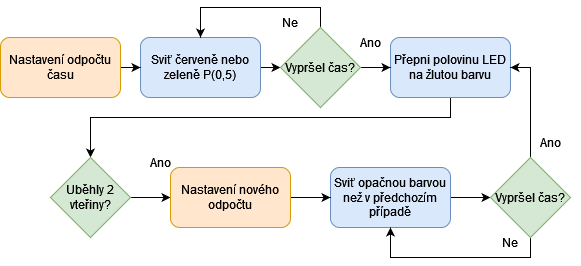
\includegraphics[scale=0.7]{obrazky/Klasicky_semafor_diagram.png}
  \end{center}
  \caption[Blokové schéma herního módu Klasický semafor]{Blokové schéma herního módu Klasický semafor.}
\end{figure}

Tento mód nahrazuje instruktora při omezování aktivit účastníků v různých herních prvcích. Může sloužit jako omezovač přístupu k surovinám ve strategických hrách, jako brána města, která se zavírá 
a otvírá a zamezuje nebo povoluje přístup k tržišti. Osvědčuje se jako faktor náhody při časově omezených úkolech, například oběh hřiště. V tomto módu mohou také Univerzální moduly náhodně řídit 
přístup do tzv. domečků - bezpečných zón, kde se lze ukrýt před útoky ostatních týmů v bojových hrách.

\section{Odpočítávání}
Tento herní mód přebírá jako parametr čas k odpočtu.

Hra je odstartována zmáčknutím středového tlačítka. Tím je spuštěn odpočet času, který byl předán tomuto módu jako parametr. V tuto chvíli všechny LED svítí zelenou barvou a postupně, po uplynutí každé 
dvanáctiny času, se přepne jedna LED na červenou. Pokud zbývá z nastaveného času poslední minuta, tak se všechny dosud zeleně svítící LED přepnou do žluté barvy a blikají v intervalu 5 sekund po dobu jedné 
sekundy. Po uplynutí natstaveného času všechny LED svítí červeně. 
Po stisku středového tlačítka je odpočet znovu nastaven a celá funkčnost se opakuje.  

\begin{figure}[!h]
  \begin{center}
    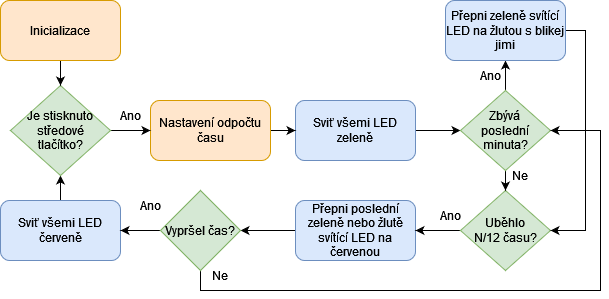
\includegraphics[scale=0.65]{obrazky/Odpocitavani_diagram.png}
  \end{center}
  \caption[Blokové schéma herního módu Odpočítávání]{Blokové schéma herního módu Odpočítávání.}
\end{figure}

Univerzální modul v tomto módu může plně nahrazovat instruktora, který hlídá penalizaci hráčů, kteří mají strávit trestný čas mimo hru. Po spuštění se jim odpočítává penalizace, aniž by na místě musel 
někdo nastavovat stopky. Toto je velmi důležitou součástí výchovy k fair-play. Univerzální modul může omezovat využitelnost herního místa nebo prvku. Například představovat odpočet do zasypání chodby, 
exploze výbušniny, nebo odjezdu vlaku. Opět platí, že se snižuje náročnost na instruktory, protože se herní místa mohou zavírat bez jejich přičinění, paralelně, nebo ve velkých vzdálenostech od sebe. 
Ve strategické hře tak například mohou simulovat postupné zavírání zdrojů surovin a přesouvat tak hru v herním prostoru.

\section{Vábnička}
Tento herní mód přebírá jako parametr počet možných barev svícení a zda má být posloupnost barev náhodná či nikoli.

Po prvním stisku se náhodně rozsvítí jedna z možných barev. Pokud je náhodnost zakázána, tak se po každém stisku středového tlačítka rozsvítí Univerzální modul barvou, která v sekvenci následuje. Pokud 
je náhodnost povolena, tak se Univerzální modul rozsvítí náhodně vygenerovanou barvou, ne však barvou, kterou svítí. V obou případech jako jedna z barev figuruje barva černá, tj. nesvítí. 

\begin{figure}[!h]
  \begin{center}
    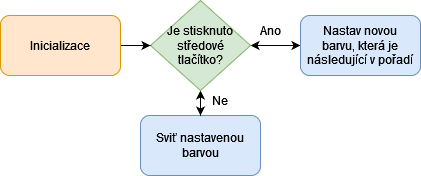
\includegraphics[scale=0.75]{obrazky/Vabnicka_diagram.png}
  \end{center}
  \caption[Blokové schéma herního módu Vábnička]{Blokové schéma herního módu Vábnička.}
\end{figure}

Univerzální modul v tomto módu může sloužit jako vizuálně atraktivní, nebo v noci použitelná, hrací kostka. V náhodném střídání barev může fungovat jako omezovač průběhu herním prostorem s podmínkou 
vlastnění klíče ve stejné barvě. V přesném střídání barev může fungovat jako stopa posledního hráče. Hráč přepne Univerzální modul na svou barvu a dává tak na vědomí, že nikdo z jeho týmu nemůže na 
stejné herní lokaci provádět herní úkony, dokud některý z jiných týmů Univerzální modul nepřepne. Pro účely nočních her to řeší omezující pravidlo - na stejném stanovišti nesmí herní mechaniku použít 
stejný tým dvakrát za sebou. Odsud jméno módu - vábí k truhle s pokladem všechny, krom vysvíceného týmu.

\chapter{Voděodolnost}
Pro zajištění voděodolnosti byl zvolen obal z průhledného silikonu. Do silikonu je DPS zalita, proto musela být navržena forma pro následné odlití. V následující části je popsán postup 
návrhu formy a následná výroba silikonového pouzdra. Nejdříve byl celý proces otestován na prototypových DPS. Po odladění bylo vše překresleno podle finální verze DPS a byly zapouzdřeny
i finální verze Univerzálního modulu.  

\section{Prototyp}
Nejprve byl vyexportován z programu KiCad 3D model celé DPS včetně všech součástek, které měly 3D model již z interní knihovny. Pro součástky, které neměly 3D model a zároveň byly důležité 
pro výsledný vzhled pouzdra, byly 3D modely dokresleny v programu SolidWorks. Pouzdra byla kreslena bez větších detailů. S přesností byla kreslena pouze kritická místa, kde součástka ovlivňuje 
rozměry pouzdra nebo kde musí procházet pouzdrem až na povrch.
  
\begin{figure}[!h]
  \begin{center}
    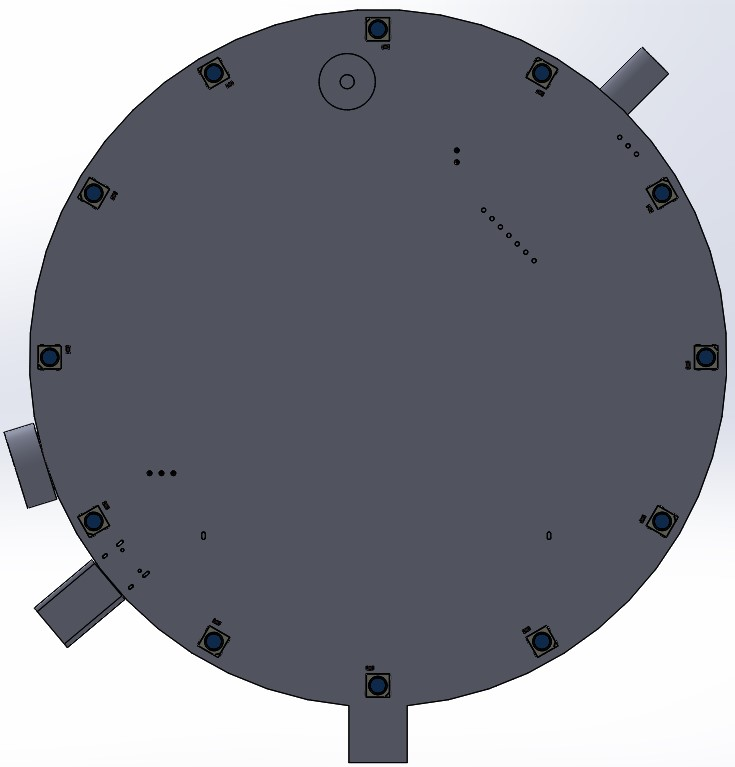
\includegraphics[scale=0.4]{obrazky/3D_model_predni.jpg}
  \end{center}
  \caption[3D model přední části DPS]{3D model přední části DPS.}
\end{figure}

Následně byl nakreslen model pouzdra, jak by mělo vypadat bez vložené DPS. Poté byla vytvořena sestava, kde byla DPS již vložené v pouzdře. Z pouzdra musely vyčnívat součásti, které nesmí být 
zality v silikonu. Nesmí být zalit USB konektor, prostřednictvím něhož je Univerzální modul napájen a programován, dále vypínač a piezo, protože by jinak nemohlo vydávat zvuk. 

Z takto vytvořeného modelu byla vytvořena forma. Byl nakreslen válec, který byl z každé strany o 3 mm větší než DPS s obalem. Poté byl použit nástroj "Kombinovat", který umožnil odečtení vytvořeného 
modelu DPS s obalem, takže vznikla dutá forma pro potřebný tvar. Následně byla forma rozdělena na 2 díly, které na sebe pasují a protínají v polovině všechny otvory tak, aby se do těchto půlek 
dala DPS zavřít.

\begin{figure}[!h]
  \begin{center}
    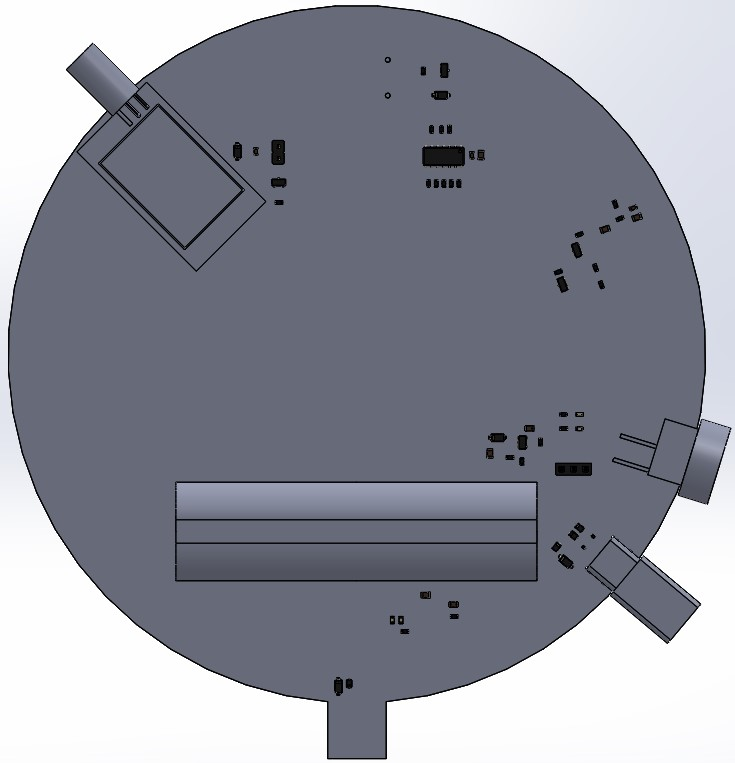
\includegraphics[scale=0.4]{obrazky/3D_model_zadni.jpg}
  \end{center}
  \caption[3D model zadní části DPS]{3D model zadní části DPS.}
\end{figure}

V předním dílu formy byl ve spodní části vytvořen otvor o průměru 2 mm pro vstřik silikonu. Ve spodní části byl proto, aby hladina silikonu postupně stoupala a nevznikaly tak při vstřiku vzduchové 
kapsy a obal byl jednolitý. Do obou dílů formy byly vytvořeny také odvzdušňovací otvory. Tyto otvory mají průměr 0,5 mm a jsou rozmístěny po cca 2 cm, aby byl zajištěn odvod vzduchu a nevznikaly tak 
v obalu vzduchové kapsy a silikon se dostal do všech potřebných míst. 

Protože silikon při tuhnutí zmenšuje svůj objem, musela být vytvořena zásobárna na silikon, který samospádem bude v průběhu tuhnutí vtékat do formy. V horní části byl tedy vytvořen zásobník, do kterého 
se při vstřikování silikonu po naplnění formy dostane silikon. Při procesu tuhnutí pak může silikon ze zásobníku přitékat do formy díky gravitaci. 

Forma na silikonový obal byla vytištěna na FMD 3D tiskárně. Nemohla být použita 3D tiskárna typu SLA, protože resin, ze kterého se v SLA tiskárnách tiskne, zabraňuje tuhnutí použitého typu silikonu. 

Před zalitím Univerzálního modulu do formy byly pomocí vteřinového lepidla zalepeny boční otvory v konektoru USB-C, aby silikon nevtekl těmito otvory dovnitř a neucpal tak tento konektor. DPS byla 
vložena do formy, utěsněna tavným lepidlem a stlačena pomocí svorek.

\begin{figure}[!h]
  \begin{center}
    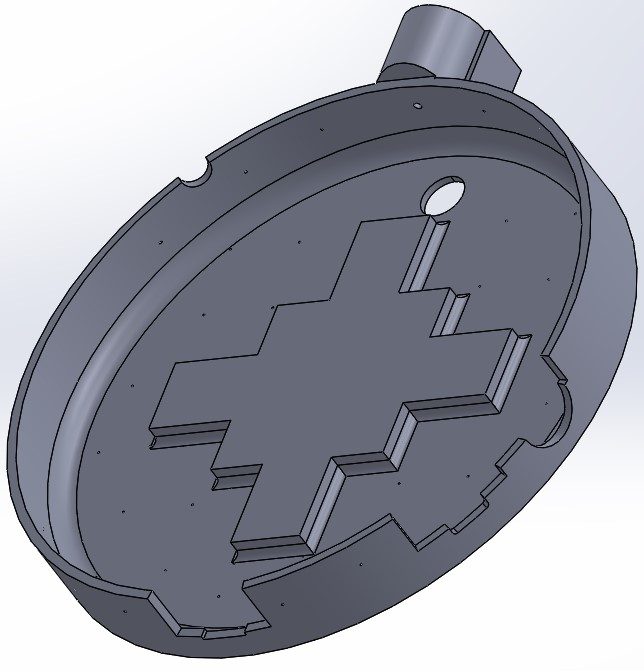
\includegraphics[scale=0.4]{obrazky/forma_predni.jpg}
  \end{center}
  \caption[3D model přední části formy]{3D model přední části formy.}
\end{figure}

%jaký typ silikonu je využit - na jaké bázi, jaké jsou jiné možnosti, výhody použitého typu 
Byl použit dvousložkový průhledný silikon GMS A30, který se míchá v poměru 1:1 \cite{silikon}. Pomocí stříkačky byl silikon vtlačen do formy. Díky tomu, že otvor byl ve spodní části formy a zásobník 
nahoře, tak hladina postupně stoupala a nemohlo dak dojít ke vzniku vzduchových kapes. Až byl naplněn i vrchní zásobník, tak byl nátlakový otvor ucpán, aby silikon nevytekl. Tuhnutí tohoto silikonu 
při pokojové teplotě trvalo asi 5 hodin \cite{silikon}. Tuhnutí silikonu vyvolává exotermní reakci a zmenšuje se tak jeho objem. Proto byl postupně to vrchního zásobníku přidávám silikon, aby byl 
Univerzální modul zalit celý. 
%fotka výsledného prototypu i s obalem

\section{Finální verze}
Pro finální verzi DPS byla vytvořena nová fomra pro odlévání silikonu. DPS finální verze má totiž jiné rozměry a součástky na ní jsou jinak naskládány. 

Pro 3D model DPS byl vytvořen ještě model posuvného vypínače, který u prototypu nebyl. Postup tvorby formy byl stejný jako u prototypu.

%možná model 
%fotka finální verze hotové i s obalem




%%% Vložení souboru 'text/zaver' se závěrem
\chapter*{Závěr}
\phantomsection
\addcontentsline{toc}{chapter}{Závěr}

Shrnutí studentské práce.


%%% Vložení souboru 'text/literatura' se seznamem zdrojů
% Pro sazbu seznamu literatury použijte jednu z následujících možností

%%%%%%%%%%%%%%%%%%%%%%%%%%%%%%%%%%%%%%%%%%%%%%%%%%%%%%%%%%%%%%%%%%%%%%%%%
%1) Seznam citací definovaný přímo pomocí prostředí literatura / thebibliography

\begin{thebibliography}{99}
	
%\bibitem{sr02/2009}
%		VUT v~Brně:
%    \emph{Úprava, odevzdávání a zveřejňování vysokoškolských kva\-li\-fi\-kač\-ních prací na VUT v~Brně}\/ [online].
%		Směrnice rektora č.\,2/2009.
%		Brno: 2009, po\-sled\-ní aktualizace 24.\,3.\,2009 [cit.\,23.\,10.\,2015].
%    Dostupné z~URL:\\
%    <\url{https://www.vutbr.cz/uredni-deska/vnitrni-predpisy-a-dokumenty/smernice-rektora-f34920/}>.

%\bibitem{CSN_ISO_690-2011}
%    \emph{ČSN ISO 690 (01 0197) Informace a dokumentace -- Pravidla pro bibliografické odkazy a citace informačních zdrojů.}
%    40 stran. Praha: Český normalizační institut, 2011.

%\bibitem{CSN_ISO_7144-1997}
%    \emph{ČSN ISO 7144 (010161) Dokumentace -- Formální úprava disertací a podobných dokumentů.}
%    24 stran. Praha: Český normalizační institut, 1997.

%\bibitem{CSN_ISO_31-11}
%    \emph{ČSN ISO 31-11 Veličiny a jednotky -- část 11: Matematické znaky a značky používané ve fyzikálních vědách a v~technice.}
%    Praha: Český normalizační institut, 1999.

%\bibitem{BiernatovaSkupa2011:CSNISO690komentar}
%    BIERNÁTOVÁ, O., SKŮPA, J.:
%    \emph{Bibliografické odkazy a citace dokumentů dle ČSN ISO 690 (01 0197) platné od 1.\,dubna 2011}\/ [online].
%    2011, poslední aktualizace 2.\,9.\,2011 [cit. 19.\,10.\,2011].
%    Dostupné z~URL:
%    \(<\)\url{http://www.citace.com/CSN-ISO-690.pdf}\(>\)
%    \(<\)\href{http://www.boldis.cz/citace/citace.html}{http://www.boldis.cz/citace/citace.html}\(>\).

%\bibitem{pravidla}
%    \emph{Pravidla českého pravopisu}.
%    Zpracoval kolektiv autorů. 1.\ vydání.
%    Olomouc: FIN PUB\-LISH\-ING, 1998. 575 s. ISBN 80-86002-40-3.

%\bibitem{Walter1999}
%	WALTER, G.\,G.; SHEN, X.
%	\emph{Wavelets and Other Orthogonal Systems}.
%	2. vyd. Boca Raton: Chapman\,\&\,Hall/CRC, 2000. 392~s. ISBN 1-58488-227-1

%\bibitem{Svacina1999IEEE}
%	SVAČINA, J.
%	Dispersion Characteristics of Multilayered Slotlines -- a Simple Approach.
%	\emph{IEEE Transactions on Microwave Theory and Techniques},
%	1999, vol.\,47, no.\,9, s.\,1826--1829. ISSN 0018-9480.

%\bibitem{RajmicSysel2002}
%    RAJMIC, P.; SYSEL, P.
%    Wavelet Spectrum Thresholding Rules.
%    In \emph{Proceedings of the International Conference Research in Telecommunication Technology},
%    Žilina: Žilina University, 2002. s.\,60--63. ISBN 80-7100-991-1.

%moje zdroje
\bibitem{akumulatory}
    ASTRA:
    \emph{Přehledné informace o typech akumulátorů}\/ [online].
    2018, poslední aktualizace 28.\,11.\,2018 [cit. 05.\,12.\,2022].
    Dostupné z~URL:
    \(<\)\url{https://www.astramodel.cz/cz/blog/prehledne-informace-o-typech-akumulatoru.html}\(>\)

\bibitem{conv_cap_but_AT42QT1070_dtsh}
    Atmel:
    \emph{Atmel AT42QT1070}\/ [online].
    2013, poslední aktualizace 05.\,2013 [cit. 9.\,11.\,2022].
    Dostupné z~URL: 
    \(<\)\url{https://ww1.microchip.com/downloads/en/DeviceDoc/Atmel-9596-AT42-QTouch-BSW-AT42QT1070_Datasheet.pdf}\(>\)

\bibitem{piezo_dtsh}
    Bestar Acoustic:
    \emph{Magnetic transducer}\/ [online].
    2003, poslední aktualizace 28.\,05.\,2003 [cit. 01.\,01.\,2023]. 
    Dostupné z~URL:
    \(<\)\url{https://www.tme.eu/Document/1ff2ab27ffcd141d4c8d7506962ac351/bmt1205xh7_5_020200.pdf}\(>\)

\bibitem{charger_dtsh}
    CONSONANCE:
    \emph{1A LiFePO4 Battery Charger CN3058E}\/ [online].
    2022, poslední aktualizace 2022 [cit. 31.\,10.\,2022].
    Dostupné z~URL: %upravit údaje o datech
    \(<\)\url{http://www.consonance-elec.com/en/static/upload/file/20220425/1650867856106004.pdf}\(>\)

\bibitem{Li-Ion}
    DUFKOVÁ, M.:
    \emph{Li-ion baterie}\/ [online].
    2015, poslední aktualizace 25.\,04.\,2015 [cit. 05.\,12.\,2022].
    Dostupné z~URL:
    \(<\)\url{https://www.3pol.cz/cz/rubriky/prakticke-informace/1677-li-ion-baterie}\(>\)

\bibitem{ESP_C3_dtsh}
    Espressif Systems:
    \emph{ESP32-C3-MINI-1}\/ [online].
    2022, poslední aktualizace 2022 [cit. 31.\,10.\,2022].
    Dostupné z~URL:
    \(<\)\url{https://www.espressif.com/sites/default/files/documentation/esp32-c3-mini-1_datasheet_en.pdf}\(>\)

\bibitem{ESP_C3_tech_ref}
    Espressif Systems:
    \emph{ESP32-C3 Technical Reference Manual}\/ [online].
    2022, poslední aktualizace 16.\,12.\,2022 [cit. 02.\,01.\,2023].
    Dostupné z~URL:
    \(<\)\url{https://www.espressif.com/sites/default/files/documentation/esp32-c3_technical_reference_manual_en.pdf}\(>\)

\bibitem{LoRa_IoT_PORT}
    IoTPORT:
    \emph{LoRaWAN - připojení do sítě IoT}\/ [online].
    2022, [cit. 28.\,12.\,2022].
    Dostupné z~URL:
    \(<\)\url{https://www.iotport.cz/lorawan-sit-pro-iot}\(>\)
 
\bibitem{shotky_dtsh}
    JCET:
    \emph{SOD-123 Plastic-Encapsulate Diodes}\/ [online].
    2015, poslední aktualizace 04.\,2015 [cit. 01.\,01.\,2023]. 
    Dostupné z~URL:
    \(<\)\url{https://datasheet.lcsc.com/lcsc/1809140216_Jiangsu-Changjing-Electronics-Technology-Co---Ltd--B5819W-SL_C8598.pdf}\(>\)

\bibitem{vib_motor_dtsh}
    LEADER:
    \emph{PRODUCT SPECIFICATION LCM1020A2945F}\/ [online].
    2021, poslední aktualizace 20.\,08.\,2021 [cit. 9.\,11.\,2022].
    Dostupné z~URL: 
    \(<\)\url{https://datasheet.lcsc.com/lcsc/2109230030_LEADER-LCM1020A2945F_C2891560.pdf}\(>\)

\bibitem{LT1930_dtsh}
    LINEAR TECHNOLOGY:
    \emph{LT1930/LT1930A}\/ [online].
    2001, poslední aktualizace 2001 [cit. 5.\,11.\,2022].
    Dostupné z~URL: 
    \(<\)\url{https://www.analog.com/media/en/technical-documentation/data-sheets/1930f.pdf}\(>\)

\bibitem{LiFePO4_malina}
    MALINA GROUP:
    \emph{Co jsou to baterie LiFePO4?}\/ [online].
    2021, poslední aktualizace 27.\,11.\,2021 [cit. 05.\,12.\,2022].
    Dostupné z~URL:
    \(<\)\url{https://malinagroup.cz/co-jsou-to-baterie-lifepo4/?gclid=Cj0KCQiAyracBhDoARIsACGFcS5eip8JqXIovxZ4ZCmRtD1Qhd0keRIml-H54afd2dTpAnDb95mwp1saAqaxEALw_wcB}\(>\)

\bibitem{MCP1640_dtsh}
    Microchip Technology Inc.:
    \emph{MCP1640/B/C/D}\/ [online].
    2010, [cit. 30.\,12.\,2022].
    Dostupné z~URL: 
    \(<\)\url{https://ww1.microchip.com/downloads/aemDocuments/documents/APID/ProductDocuments/DataSheets/MCP1640-Family-Data-Sheet-DS20002234E.pdf}\(>\)

\bibitem{LoRa_eman}
    PECH, J.:
    \emph{IOT TECHNOLOGIE: LORA A LORAWAN (3/5)}\/ [online].
    2019, poslední aktualizace 19.\,02.\,2019 [cit. 28.\,12.\,2022].
    Dostupné z~URL:
    \(<\)\url{https://www.eman.cz/blog/iot-technologie-lora-a-lorawan-3-5/}\(>\)

\bibitem{rezistorova_rada}
    Radioklub OK1KVK:
    \emph{Elektrotechnické řady hodnot E3, E6, E12, E24}\/ [online].
    2011, poslední aktualizace 25.\,05.\,2011 [cit. 31.\,10.\,2022].
    Dostupné z~URL: 
    \(<\)\url{https://ok1kvk.cz/clanek/2011/elektrotechnicke-rady-hodnot-e3-e6-e12-e24/}\(>\)

\bibitem{Bezdrat_muni}
    RNDr. Michal Černý, Ph.D.:
    \emph{Bezdrátové protokoly - základní přehled}\/ [online].
    2014, poslední aktualizace 16.\,01.\,2014 [cit. 12.\,11.\,2022].
    Dostupné z~URL: 
    \(<\)\url{https://is.muni.cz/el/1421/jaro2013/VIKMB15/um/Bezdratove_protokoly.pdf}\(>\)
    
\bibitem{Sigfox_cz}
    Sigfox:
    \emph{Sigfox.cz}\/ [online].
    2021 [cit. 03.\,01.\,2023].
    Dostupné z~URL: 
    \(<\)\url{https://sigfox.cz/cs}\(>\)

\bibitem{ZigBee_smart}
    Smart-switch:
    \emph{ZIGBEE VS WIFI, CO JE LEPŠÍ?}\/ [online].
    2021, poslední aktualizace 10.\,03.\,2021 [cit. 13.\,11.\,2022].
    Dostupné z~URL: 
    \(<\)\url{https://www.smart-switch.cz/blog/zigbee-vs-wifi-co-je-lepsi/}\(>\)

\bibitem{Mech_tl_princip}
    SSP Brno:
    \emph{Klávesnice}\/ [online].
    2019, poslední aktualizace 19.\,02.\,2019 [cit. 29.\,12.\,2022]. %datum poslední aktualizace - upravit
    Dostupné z~URL:
    \(<\)\url{https://moodle.sspbrno.cz/pluginfile.php/11562/mod_resource/content/2/cast2_06_klavesnice.pdf}\(>\)

\bibitem{civka_dtsh}
    Sumida:
    \emph{SMD Power Inductor CDRH3D18}\/ [online].
    2017, poslední aktualizace 09.\,01.\,2017 [cit. 01.\,01.\,2023]. 
    Dostupné z~URL:
    \(<\)\url{https://datasheet.lcsc.com/lcsc/1809140821_Sumida-CDRH3D18NP-4R7NC_C167273.pdf}\(>\)

\bibitem{olovene}
    ŠPINA, M.:
    \emph{Olověné baterie: Stálice na poli akumulace již více než půldruhého století}\/ [online].
    2021, poslední aktualizace 17.\,06.\,2021 [cit. 05.\,12.\,2022].
    Dostupné z~URL:
    \(<\)\url{https://oenergetice.cz/akumulace-energie/olovene-baterie-stalice-poli-akumulace-jiz-vice-nez-puldruheho-stoleti}\(>\)

\bibitem{USB-C}
    USB 3.0 Promoter Group:
    \emph{Universal Serial Bus Type-C Cable and Connector Specification}\/ [online].
    2019, poslední aktualizace 08.\,2019 [cit. 01.\,01.\,2023]. 
    Dostupné z~URL:
    \(<\)\url{https://www.usb.org/sites/default/files/USB%20Type-C%20Spec%20R2.0%20-%20August%202019.pdf}\(>\)

\bibitem{LiFePO4_smart}
    VANDA, D.:
    \emph{LiFePO4 baterie: V čem jsou lepší než Li-Ion či Li-Pol a proč je chtít?}\/ [online].
    2022, poslední aktualizace 05.\,10.\,2022 [cit. 05.\,12.\,2022].
    Dostupné z~URL:
    \(<\)\url{https://insmart.cz/lifepo4-baterie-v-cem-jsou-lepsi-nez-li-ion-ci-li-pol-a-co-nabizi/}\(>\)

\bibitem{PrincipKapTl}
    VOJÁČEK, A.:
    \emph{Pravidla pro konstrukci kapacitních dotykových tlačítek mTouch}\/ [online].
    2008, poslední aktualizace 13.\,12.\,2008 [cit. 26.\,10.\,2022].
    Dostupné z~URL:
    \(<\)\url{https://automatizace.hw.cz/pravidla-pro-konstrukci-kapacitnich-dotykovych-tlacitek-mtouch}\(>\)

\bibitem{WS2812C_dtsh}
    Worldsemi:
    \emph{WS2812C Intelligent control LED}\/ [online].
    2007, poslední aktualizace 2007 [cit. 10.\,11.\,2022].
    Dostupné z~URL: 
    \(<\)\url{https://datasheet.lcsc.com/lcsc/1810231210_Worldsemi-WS2812C_C114587.pdf}\(>\)

\bibitem{Sigfox_Zooco}
    ZOOCO:
    \emph{Co je to síť Sigfox?}\/ [online].
    2023 [cit. 03.\,01.\,2023].
    Dostupné z~URL: 
    \(<\)\url{https://zooco.beyondpage.info/napoveda-zooco/faq/sigfox/co-je-to-sit-sigfox}\(>\)

\end{thebibliography}


%%%%%%%%%%%%%%%%%%%%%%%%%%%%%%%%%%%%%%%%%%%%%%%%%%%%%%%%%%%%%%%%%%%%%%%%%
%%2) Seznam citací pomocí BibTeXu
%% Při použití je nutné v TeXnicCenter ve výstupním profilu aktivovat spouštění BibTeXu po překladu.
%% Definice stylu seznamu
%\bibliographystyle{unsrturl}
%% Pro českou sazbu lze použít styl czechiso.bst ze stránek
%% http://www.fit.vutbr.cz/~martinek/latex/czechiso.tar.gz
%%\bibliographystyle{czechiso}
%% Vložení souboru se seznamem citací
%\bibliography{text/literatura}
%
%% Následující příkaz je pouze pro ukázku sazby literatury při použití BibTeXu.
%% Způsobí citaci všech zdrojů v souboru literatura.bib, i když nejsou citovány v textu.
%\nocite{*}

%%% Vysázení seznamu obrázků
% (vynechejte, pokud máte dva nebo méně obrázků)
\listoffigures

%%% Vysázení seznamu tabulek
% (vynechejte, pokud máte dvě nebo méně tabulek)
\listoftables

%%% Vysázení seznamu výpisů kódu
% (vynechejte, pokud máte dva nebo méně výpisů)
\lstlistoflistings

%%% Vložení souboru 'text/zkratky' se seznam použitých symbolů, veličin a zkratek
\cleardoublepage
\chapter*{\listofabbrevname}
\phantomsection
\addcontentsline{toc}{chapter}{\listofabbrevname}

\begin{acronym}[KolikMista]

	\acro{AD}{Analog to Digital - analogově-digitální}
	\acro{dB}{decibel - jednotka intenzity zvuku}
	\acro{DPS}{Deska plošného spoje}
	\acro{EMC}{Elektromagnetická kompatibilita}
	\acro{FDM}{Fused deposition modeling -  metoda 3D tisku pomocí taveného nanášení}
	\acro{GND}{Ground - nulový potenciál}
	\acro{GPIO}{General Purpose Input/Output - vstupně-výstupní piny}
	\acro{IoT}{Internet of Things}
	\acro{$I^2C$}{Inter-Integrated Circuit - multi-masterová sériová komunikační sběrnice}
	\acro{LED}{Light-Emitting Diode - dioda emitující světlo}
	\acro{LoRa}{Long Range Radio}
	\acro{LoRaWAN}{Long Range Wide Area Network}
	\acro{MCU}{Mikrokontrolér}
	\acro{NFC}{Near Field Communication - typ bezdrátové komunikace}
	\acro{RF}{Rádiová frekvence}
	\acro{ROM}{Read-Only Memory - typ elektronické paměti}
	\acro{SLA}{Stereolitografie}
	\acro{SPI}{Serial Peripheral Interface - sériové komunikační periferní rozhraní}
	\acro{UART}{Universal asynchronous receiver-transmitter - komunikační sběrnice}
	\acro{USB}{Universal Serial Bus - univerzální komunikační sériová sběrnice}
	\acro{WiFi}{Wireless Fidelity}

	%\acro{zkDummy}
	%	[KolikMista]
	%	{pouze ukázka vyhrazeného místa}

	%\acro{symfvz}						% název
	%	[\ensuremath{f_\textind{vz}}] % symbol
	%	{vzorkovací kmitočet}					% popis

\end{acronym}


%%% Začátek příloh
\appendix

%%% Vysázení seznamu příloh
% (vynechejte, pokud máte dvě nebo méně příloh)
\listofappendices

%%% Vložení souboru 'text/prilohy' s přílohami
% Obvykle je přítomen alespoň popis co najdeme na přiloženém médiu
\chapter{Schéma zapojení elektroniky}

\begin{figure}[!h]
	\begin{center}
	  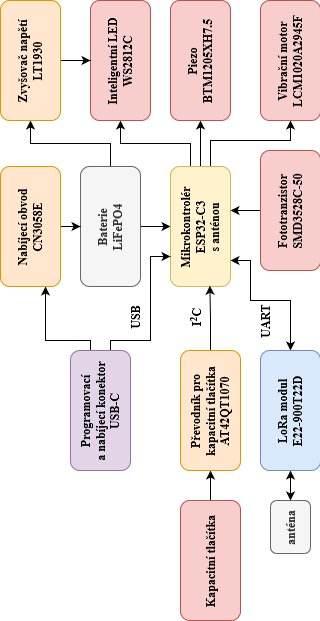
\includegraphics[scale=1.2]{obrazky/blokove_schema_finalni_verze_priloha.png}
	\end{center}
	\caption[Blokové schéma zapojení elektroniky Univerzálního modulu]{Blokové schéma zapojení elektroniky Univerzálního modulu.}
\end{figure}

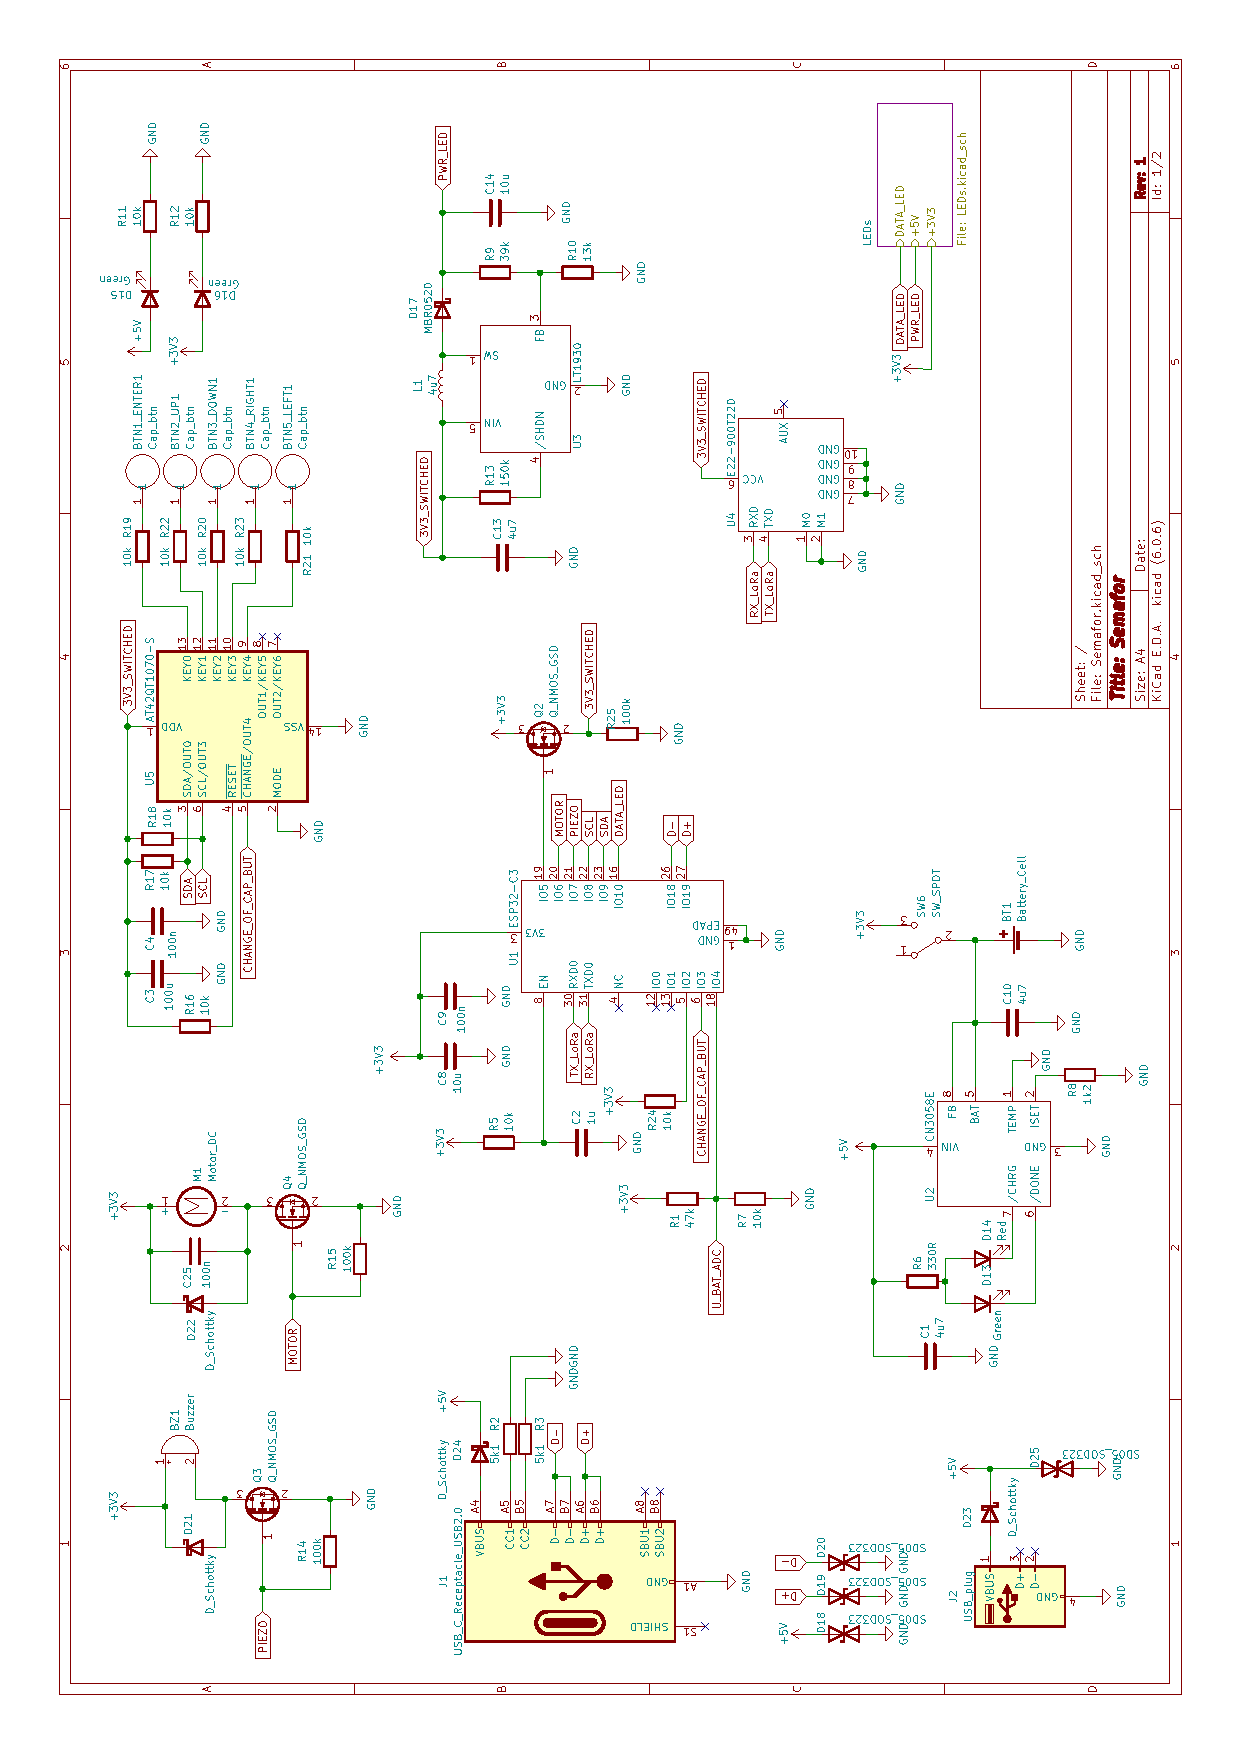
\includepdf[pages=1]{prilohy/schema_zapojeni}
\includepdf[pages=2]{prilohy/schema_zapojeni}

%přidat DPS a její výrobní podklady

\chapter{Uživatelský manuál}
Univerzální modul je zapnut pomocí posuvného vypínače. Zapnutí je indikováno rozsvícením LED uprostřed Univerzálního modulu. Při zapínání Univerzálního modulu nesmí být stisknuto žádné tlačítko. Po zapnutí je načten 
poslední používaný mód. 

Po dobu 5 minut od zapnutí je možné přepnout Univerzální modul do konfiguračního módu. Tento mód je k dispozici pomocí současného stisku horního a spodního tlačítka. Konfigurační mód je signalizován blikáním všech 
LED modře. Po zapnutí tohoto módu je zapotřebí telefon 
nebo notebook, který má možnost připojit se k WiFi síti. V zařízení je zapotřebí najít WiFi síť s názvem UniverzalniModul. Připojení proběhne po zadání hesla univerzalnimodul. Po připojení k této WiFi síti přejďete 
do internetového vyhledávače. Do něj napište IP adresu Univerzálního modulu, tj. 192.168.4.1. 

Zobrazí se webová stránka s konfiguračním menu Univerzálního modulu. Zde si můžete najít konkrétní hru i s jejím popisem. Pokud lze u dané hry nastavit nějaké parametry, jako je například počet hrajících týmů apod., tak 
jsou u této hry místa, kam lze daný parametr vyplnit. Pro nastavení dané hry stiskněte tlačítko dané hry. V tuto chvíli se spustí daný mód na všech Univerzálních modulech, 
které jsou v danou chvíli zapnuty, v blízkosti konfigurovaného Univerzálního modulu a neuběhlo u nich 5 minut od jejich zapnutí. Po restartu konfigurovaného Univerzálního modulu je i u něj spuštěn nastavený mód. 

Tímto způsobem lze konfigurovat až 9 Univerzálních modulů současně. 

\chapter{Příklad outdoorové aktivity s využitím \\Univerzálního modulu}
%outdoorových aktivit


\iffalse
\section{Příkazy pro sazbu veličin a jednotek}

\begin{table}[!h]
  \caption[Přehled příkazů]{Přehled příkazů pro matematické prostředí }
  \begin{center}
  	\small
	  \begin{tabular}{|c|c|c|c|}
	    \hline
	    Příkaz    						& Příklad 					& Zdroj příkladu  							& Význam  \\
	    \hline\hline
	    \verb|\textind{...}|	& $\beta_\textind{max}$ 	& \verb|$\beta_\textind{max}$|	& textový index \\
	    \hline
	    \verb|\const{...}| 		& $\const{U}_\textind{in}$ 				& \verb|$\const{U}_\textind{in}$|		& konstantní veličina \\
	    \hline
	    \verb|\var{...}| 		& $\var{u}_\textind{in}$ & \verb|$\var{u}_\textind{in}$| & proměnná veličina \\
	    \hline
	    \verb|\complex{...}| 	& $\complex{u}_\textind{in}$ & \verb|$\complex{u}_\textind{in}$| & komplexní veličina \\
	    \hline
	    \verb|\vect{...}| 		& $\vect{y}$ 						& \verb|$\vect{y}$| & vektor \\
	    \hline
	    \verb|\mat{...}| 	& $\mat{Z}$ 						& \verb|$\mat{Z}$| & matice \\
	    \hline
	    \verb|\unit{...}| 		& $\unit{kV}$ 						& \verb|$\unit{kV}$|\quad či\ \, \verb|\unit{kV}| & jednotka \\
	    \hline
	  \end{tabular}
  \end{center}
\end{table}



\newpage
\section{Příkazy pro sazbu symbolů}

\begin{itemize}
  \item
    \verb|\E|, \verb|\eul| -- sazba Eulerova čísla: $\eul$,
  \item
    \verb|\J|, \verb|\jmag|, \verb|\I|, \verb|\imag| -- sazba imaginární jednotky: $\jmag$, $\imag$,
  \item
    \verb|\dif| -- sazba diferenciálu: $\dif$,
  \item
    \verb|\sinc| -- sazba funkce: $\sinc$,
  \item
    \verb|\mikro| -- sazba symbolu mikro stojatým písmem%
			\footnote{znak pochází z~balíčku \texttt{textcomp}}: $\mikro$,
	\item
		\verb|\uppi| -- sazba symbolu $\uppi$
			(stojaté řecké pí, na rozdíl od \verb|\pi|, což sází $\pi$).
\end{itemize}

Všechny symboly jsou určeny pro matematický mód, vyjma \verb|\mikro|, jenž je\\ použitelný rovněž v~textovém módu.
$\upmikro$


\chapter{Druhá příloha}

Pro sazbu vektorových obrázků přímo v~\LaTeX{}u je možné doporučit balíček \href{https://www.ctan.org/pkg/pgf}{\texttt{TikZ}}.
Příklady sazby je možné najít na \href{http://www.texample.net/tikz/examples/}{\TeX{}ample}.
Pro vyzkoušení je možné použít programy QTikz nebo TikzEdt.




%\chapter{Příklad sazby zdrojových kódů}

%\section{Balíček \texttt{listings}}

%Pro vysázení zdrojových souborů je možné použít balíček \href{https://www.ctan.org/pkg/listings}{\texttt{listings}}.
%Balíček zavádí nové prostředí \texttt{lstlisting} pro sazbu zdrojových kódů, jako například:
%
%\begin{lstlisting}[language={[LaTeX]TeX}]
%\section{Balíček lstlistings}
%Pro vysázení zdrojových souborů je možné použít
%	balíček \href{https://www.ctan.org/pkg/listings}%
%	{\texttt{listings}}.
%Balíček zavádí nové prostředí \texttt{lstlisting} pro
%	sazbu zdrojových kódů.
%\end{lstlisting}
%
%Podporuje množství programovacích jazyků.
%Kód k~vysázení může být načítán přímo ze zdrojových souborů.
%Umožňuje vkládat čísla řádků nebo vypisovat jen vybrané úseky kódu.
%Např.:

%\noindent
%Zkratky jsou sázeny v~prostředí \texttt{acronym}:
%\label{lst:zkratky}
%\lstinputlisting[language={[LaTeX]TeX},nolol,numbers=left, firstnumber=6, firstline=6,lastline=6]{text/zkratky.tex}
%
%Šířka textu volitelného parametru \verb|KolikMista| udává šířku prvního sloupce se zkratkami.
%Proto by měla být zadávána nejdelší zkratka nebo symbol.

%\shorthandoff{-}
%\lstinputlisting[language={[LaTeX]TeX},frame=single,caption={Ukázka sazby zkratek},label=lst:symfvz,numbers=left,linerange={bsymfvz-\%\%\%\ esymfvz},includerangemarker=false]{text/zkratky.tex}
%\shorthandon{-}

%\noindent
%Ukončení seznamu je provedeno ukončením prostředí:
%\lstinputlisting[language={[LaTeX]TeX},nolol,numbers=left,firstnumber=26,linerange=26]{text/zkratky.tex}

%\vspace{\fill}

%\noindent
%{\bf Poznámka k~výpisům s~použitím volby jazyka \verb|czech| nebo \verb|slovak|:}\newline
%Pokud Váš zdrojový kód obsahuje znak spojovníku \verb|-|, pak překlad může skončit chybou.
%Ta je způsobená tím, že znak \verb|-| je v~českém nebo slovenském nastavení balíčku \verb|babel| tzv.\ aktivním znakem.
%Přepněte znak \verb|-| na neaktivní příkazem \verb|\shorthandoff{-}| těsně před výpisem a hned za ním jej vraťte na aktivní příkazem \verb|\shorthandon{-}|.
%Podobně jako to je ukázáno ve zdrojovém kódu šablony.


%\clearpage

%\section{Výpis kódu prostředí Matlab}
%Na výpisu \ref{lst:priklad.vypis.kodu.Matlab} naleznete příklad kódu pro Matlab, na výpisu \ref{lst:priklad.vypis.kodu.C} zase pro jazyk~C.

%\lstnewenvironment{matlab}[1][]{%
%\iflanguage{czech}{\shorthandoff{-}}{}%
%\iflanguage{slovak}{\shorthandoff{-}}{}%
%\lstset{language=Matlab,numbers=left,#1}%
%}{%
%\iflanguage{slovak}{\shorthandon{-}}{}%
%\iflanguage{czech}{\shorthandon{-}}{}%
%}

%\begin{matlab}[frame=single,float=htbp,caption={Příklad Schur-Cohnova testu stability v~prostředí Matlab.},label=lst:priklad.vypis.kodu.Matlab,numberstyle=\scriptsize, numbersep=7pt]
%% Priklad testovani stability filtru

% koeficienty polynomu ve jmenovateli
%a = [ 5, 11.2, 5.44, -0.384, -2.3552, -1.2288];
%disp( 'Polynom:'); disp(poly2str( a, 'z'))

%disp('Kontrola pomoci korenu polynomu:');
%zx = roots( a);
%if( all( abs( zx) < 1))
%    disp('System je stabilni')
%else
%    disp('System je nestabilni nebo na mezi stability');
%end

%disp(' '); disp('Kontrola pomoci Schur-Cohn:');
%ma = zeros( length(a)-1,length(a));
%ma(1,:) = a/a(1);
%for( k = 1:length(a)-2)
%    aa = ma(k,1:end-k+1);
%    bb = fliplr( aa);
%    ma(k+1,1:end-k+1) = (aa-aa(end)*bb)/(1-aa(end)^2);
%end

%if( all( abs( diag( ma.'))))
%    disp('System je stabilni')
%else
%    disp('System je nestabilni nebo na mezi stability');
%end
%\end{matlab}

%\noindent
%\begin{minipage}{\linewidth}


%\section{Výpis kódu jazyka C}

\begin{lstlisting}[frame=single,numbers=right,caption={Příklad implementace první kanonické formy v~jazyce C.},label=lst:priklad.vypis.kodu.C,basicstyle=\ttfamily\small, keywordstyle=\color{black}\bfseries\underbar,]
// první kanonická forma
short fxdf2t( short coef[][5], short sample)
{
	static int v1[SECTIONS] = {0,0},v2[SECTIONS] = {0,0};
	int x, y, accu;
	short k;

	x = sample;
	for( k = 0; k < SECTIONS; k++){
		accu = v1[k] >> 1;
		y = _sadd( accu, _smpy( coef[k][0], x));
		y = _sshl(y, 1) >> 16;

		accu = v2[k] >> 1;
		accu = _sadd( accu, _smpy( coef[k][1], x));
		accu = _sadd( accu, _smpy( coef[k][2], y));
		v1[k] = _sshl( accu, 1);

		accu = _smpy( coef[k][3], x);
		accu = _sadd( accu, _smpy( coef[k][4], y));
		v2[k] = _sshl( accu, 1);

		x = y;
	}
	return( y);
}
\end{lstlisting}
\end{minipage}







%\chapter{Obsah elektronické přílohy}
%Elektronická příloha je často nedílnou součástí semestrální nebo závěrečné práce.
%Vkládá se do informačního systému VUT v~Brně ve vhodném formátu (ZIP, PDF\,\dots).

%Nezapomeňte uvést, co čtenář v~této příloze najde.
%Je vhodné okomentovat obsah každého adresáře, specifikovat, který soubor obsahuje důležitá nastavení, který soubor je určen ke spuštění, uvést nastavení kompilátoru atd.
%Také je dobře napsat, v~jaké verzi software byl kód testován (např.\ Matlab 2018b).
%Pokud bylo cílem práce vytvořit hardwarové zařízení,
%musí elektronická příloha obsahovat veškeré podklady pro výrobu (např.\ soubory s~návrhem DPS v~Eagle).

%Pokud je souborů hodně a jsou organizovány ve více složkách, je možné pro výpis adresářové struktury použít balíček \href{https://www.ctan.org/pkg/dirtree}{\texttt{dirtree}}.

%\bigskip

%{\small
%
%\dirtree{%.
%.1 /\DTcomment{kořenový adresář přiloženého archivu}.
%.2 logo\DTcomment{loga školy a fakulty}.
%.3 BUT\_abbreviation\_color\_PANTONE\_EN.pdf.
%.3 BUT\_color\_PANTONE\_EN.pdf.
%.3 FEEC\_abbreviation\_color\_PANTONE\_EN.pdf.
%.3 FEKT\_zkratka\_barevne\_PANTONE\_CZ.pdf.
%.3 UTKO\_color\_PANTONE\_CZ.pdf.
%.3 UTKO\_color\_PANTONE\_EN.pdf.
%.3 VUT\_barevne\_PANTONE\_CZ.pdf.
%.3 VUT\_symbol\_barevne\_PANTONE\_CZ.pdf.
%.3 VUT\_zkratka\_barevne\_PANTONE\_CZ.pdf.
%.2 obrazky\DTcomment{ostatní obrázky}.
%.3 soucastky.png.
%.3 spoje.png.
%.3 ZlepseneWilsonovoZrcadloNPN.png.
%.3 ZlepseneWilsonovoZrcadloPNP.png.
%.2 pdf\DTcomment{pdf stránky generované informačním systémem}.
%.3 student-desky.pdf.
%.3 student-titulka.pdf.
%.3 student-zadani.pdf.
%.2 text\DTcomment{zdrojové textové soubory}.
%.3 literatura.tex.
%.3 prilohy.tex.
%.3 reseni.tex.
%.3 uvod.tex.
%.3 vysledky.tex.
%.3 zaver.tex.
%.3 zkratky.tex.
%.2 navod-sablona\_FEKT.pdf\DTcomment{návod na používání šablony}.
%.2 sablona-obhaj.tex\DTcomment{hlavní soubor pro sazbu prezentace k~obhajobě}.
%.2 readme.txt\DTcomment{soubor s~popisem obsahu CD}.
%.2 sablona-prace.tex\DTcomment{hlavní soubor pro sazbu kvalifikační práce}.
%.2 thesis.sty\DTcomment{balíček pro sazbu kvalifikačních prací}.
%}
%}

\fi

\end{document}